\documentclass[10pt,a4paper]{article}
\usepackage[margin=0.75in]{geometry}
\usepackage[T1]{fontenc}
\usepackage[utf8]{inputenc}
\usepackage{lmodern,amsmath,amssymb,booktabs,array,enumitem}
\usepackage[expansion=false]{microtype}
\usepackage{csquotes}
\usepackage{xurl,hyperref,pdflscape,tabularx,algorithm,algpseudocode,graphicx,tikz,xcolor}
\usepackage[section]{placeins}
\hypersetup{hidelinks}
\newcolumntype{Y}{>{\raggedright\arraybackslash}X}
\newcolumntype{L}[1]{>{\raggedright\arraybackslash}p{#1}}
\newcommand{\NA}{\mathrm{N/A}}
\newcommand{\CE}{\operatorname{CE}}
\newcommand{\sumitem}[2]{\noindent\textbf{#1:} #2\par}
\newcommand{\why}[1]{\par\noindent\colorbox{black!5}{\parbox{\dimexpr\linewidth-2\fboxsep}{\small\textbf{Why (literature basis):} #1}}\par}
\setlength{\parindent}{0pt}
\setlength{\parskip}{4pt}
\setlength{\tabcolsep}{3pt}
\renewcommand{\arraystretch}{1.12}
\setlist{nosep,leftmargin=*}

\title{\textbf{Computer Networks --- Research Project}\\[4pt]
\large Phase 2: Extended Literature Review and Research Methodology\\[8pt]
\Large Poisoning, Retention and Legitimate Adaptation\\in Federated Continual Intrusion Detection}
\author{Saneedullah (23I-2568) \qquad Ahmed Bilal (23I-2581)}
\date{October 2026}

\begin{document}
\maketitle

\begin{abstract}
Intrusion detection systems (IDS) must keep learning new attack families without forgetting old ones, and they are increasingly trained \emph{federally}, across several organizations that never share raw traffic. Our Phase 1 review found that continual-learning security methods are tested almost only with honest participants. In Phase 2 we extend the review with ten additional 2025--2026 studies and confirm a sharper gap: continual-learning IDS assume clean labels and honest clients, while federated poisoning defences are evaluated only on a fixed set of attack classes, and those defences can discard honest but rare or new evidence. We propose a controlled study on CICIDS2017 in which five federated clients learn four successive attack-family stages with fine-tuning, an EWC-style regulariser or DER++ replay. One client receives poisoned labels (DoS-Hulk relabelled as benign) during the second stage only. We measure (i) immediate damage to the poisoned family, (ii) whether the damage persists after the attacker withdraws, and (iii) how a class-aware admission rule trades off poisoning damage against the learning of new attack families, compared with an equally sized global filter. Twelve paired seeds and pre-declared statistical tests support the analysis. This document reports a research design; all performance figures quoted belong to the cited studies.
\end{abstract}
\noindent\textbf{Keywords:} continual learning; federated learning; intrusion detection; label poisoning; replay memory; legitimate adaptation.

%=====================================================================
\section{Introduction and Scope}
Network attacks change continuously. An IDS that is retrained on each new attack family tends to forget earlier families (\emph{catastrophic forgetting}); continual-learning (CL) methods such as regularisation and replay reduce this problem. At the same time, privacy rules push organizations towards \emph{federated learning} (FL), where each site trains locally and only model updates are combined. Combining the two creates a security question that neither field answers on its own: what happens when one participant's labels are wrong \emph{while} the shared model is learning a new attack family, and does a defence that filters suspicious data also block the legitimate new family it should learn?

Our Phase 1 report \cite{phase1} studied three 2026 papers on CL for network security \cite{ge,wu,luo} and identified three gaps: old or synthetic evaluation data, no testing against attackers who target the adaptation mechanism, and no measured deployment cost. Phase 2 keeps Phase 1 unchanged and builds on it. Table~\ref{tab:phase1link} shows how each Phase 1 gap is carried forward.

\begin{table}[htbp]
\centering\footnotesize
\caption{How the Phase 1 gaps carry into Phase 2.}
\label{tab:phase1link}
\begin{tabularx}{\linewidth}{L{4.6cm}L{3.3cm}Y}
\toprule
Phase 1 gap & Phase 2 status & Reason\\
\midrule
Gap 1: old, narrow or synthetic evaluation data & Narrowed & Real public captures (CICIDS2017) with an external CICIoT2023 check; synthetic RF data dropped.\\
Gap 2: no attacker targeting the continual-learning mechanism & \textbf{Retained as the core} & Becomes Gaps G1 and G2 below: poisoning during class acquisition and defence side-effects.\\
Gap 3: no measured runtime or deployment cost & Partly retained & We measure CPU time, memory and update bytes; physical edge-device energy is deferred (no hardware available).\\
\bottomrule
\end{tabularx}
\end{table}

We ask three research questions:
\begin{itemize}
\item \textbf{RQ1:} How do fine-tuning, an EWC-style regulariser and DER++ replay differ in the damage a poisoned stage causes to the targeted attack family, both immediately and after the attacker withdraws?
\item \textbf{RQ2:} Compared with a global filter that admits the same number of samples, how does a class-aware admission rule change the trade-off between poisoning damage and the learning of new attack families?
\item \textbf{RQ3:} Which memory and selection mechanisms explain the differences, and what computation and communication do they cost?
\end{itemize}
Throughout this document, page numbers cited for the reviewed articles refer to the PDF pages of each article.

%=====================================================================
\section{Deliverable 1: Extended Literature Review}

\subsection{Search Strategy and Selection Criteria}
We searched for studies that combine at least two of: intrusion detection, continual or incremental learning, federated learning, and poisoning. Sources were the Crossref publication index (journal articles dated 2025-01-01 to 2026-12-31; queries such as \emph{federated continual learning intrusion detection}, \emph{poisoning attack federated intrusion detection defense} and \emph{class incremental intrusion detection replay}), author and publisher pages, and the references of our Phase 1 papers. Each candidate had to satisfy the course criteria: published in 2025--2026; an original research article; a Q1--Q2 journal or a peer-reviewed conference; directly relevant; with an identifiable method, dataset and evaluation. We kept only papers whose \emph{complete} text we could read, because a critical analysis needs the full experimental details. One formally eligible candidate was rejected after full reading because its dataset was synthetic and unpublished and its results came from a single run. Table~\ref{tab:corpus} lists the ten selected papers. Journal quartiles follow the Clarivate Journal Citation Reports 2024 edition (released June 2025) \cite{clarivate}.

\begin{table}[htbp]
\centering\footnotesize
\caption{The ten additional papers reviewed in Phase 2. CS-IS: Computer Science, Information Systems.}
\label{tab:corpus}
\begin{tabularx}{\linewidth}{L{0.55cm}L{3.3cm}Y L{0.8cm}L{2.9cm}L{2.6cm}}
\toprule
ID & Study & Venue (publisher) & Year & Ranking & Main topic\\
\midrule
P4 & Carillo et al. \cite{carillo} & IEEE Trans. Network and Service Management (IEEE) & 2026 & Q1, CS-IS & Federated class-incremental IDS\\
P5 & Lavaur et al. \cite{lavaur} & Computers \& Security (Elsevier) & 2025 & Q1, CS-IS & Label flipping in federated IDS\\
P6 & Fuhrman et al. \cite{cnd} & ACM/IEEE Design Automation Conf. (DAC) & 2025 & Peer-reviewed conference & Continual novelty detection\\
P7 & Sameera et al. \cite{wei} & J. Information Security and Applications (Elsevier) & 2025 & Q2, CS-IS & Poisoning defence for federated IDS\\
P8 & Cerasuolo et al. \cite{cerasuolo} & Computer Networks (Elsevier) & 2025 & Q1, CS-IS & Class-incremental IDS benchmark\\
P9 & Guo et al. \cite{guo} & Future Internet (MDPI) & 2025 & Q2, CS-IS & Continual IDS, memory selection\\
P10 & Latif and Djenouri \cite{amm} & Sensors (MDPI) & 2026 & Q2 & Robust hierarchical federated IDS\\
P11 & Banbhrani et al. \cite{flzt} & Electronics (MDPI) & 2026 & Q2 & Trust-aware federated IDS\\
P12 & Abhijit et al. \cite{rare} & Scientific Reports (Nature Portfolio) & 2025 & Q1 & Federated rare/new attack classes\\
P13 & Nguyen and Park \cite{elgnn} & Electronics (MDPI) & 2025 & Q2 & EWC-based continual IDS\\
\bottomrule
\end{tabularx}
\end{table}
% VERIFY before submission: confirm the JCR/SJR quartiles of Sensors, Electronics and Scientific Reports on the journal profiles.

\subsection{Critical Summaries of the Ten Additional Papers}
Each summary follows the same structure as Phase 1: what the paper does, how it was evaluated, what it found, the limitations the authors state, the limitations we identify, and why it matters for our study.

\subsubsection*{P4 --- A Federated and Incremental Network Intrusion Detection System for IoT Emerging Threats (Carillo et al., 2026)}
\sumitem{Problem and method}{Clients must learn new attack classes that appear only at some sites, without forgetting old ones. The authors combine federated optimisers (FedAvg, FedProx, FedDyn) with class-incremental methods that use rehearsal, distillation and bias correction (BiC+, MEMENTO+). Inputs are matrices of the first ten packets of each bidirectional flow, with IP addresses and ports removed.}
\sumitem{Data and setup}{TON\_IoT, IoT-NID and Edge-IIoTset; scenarios with two and five clients, each contributing a disjoint new attack (p.~1).}
\sumitem{Key results}{The best setting (FedProx with MEMENTO+, 100 rounds, five clients on TON\_IoT) reaches old/new/all-class F1 of 79.05/68.10/74.49\% (Table IV).}
\sumitem{Author-stated limitations}{Federated class-incremental learning retains old knowledge but has difficulty integrating new attacks; future work lists improved robustness against adversarial threats (Sec.~VI, p.~15).}
\sumitem{Our critique}{All clients are honest; the gap between old-class and new-class F1 shows that acquisition, not retention, is the weak point, so any defence that rejects new-class data would make it worse.}
\sumitem{Relevance}{Clean reference for federated class acquisition and for reporting old and new classes separately.}

\subsubsection*{P5 --- Investigating the Impact of Label-Flipping Attacks against Federated Learning for Collaborative Intrusion Detection (Lavaur et al., 2025)}
\sumitem{Problem and method}{How damaging are targeted and untargeted label flips in federated IDS? A binary multilayer perceptron with two hidden layers of 128 units (pp.~9--10) is trained with FedAvg while the share of malicious clients, the flip rate, attack timing and data heterogeneity are varied.}
\sumitem{Data and setup}{NetFlow-v2 versions of CSE-CIC-IDS2018 and UNSW-NB15; ten clients; 10,670 runs.}
\sumitem{Key results}{With one attacker among ten clients, relative attack success stays below 0.1 even when all its local labels are flipped (Sec.~5.4, Fig.~10); damage grows with attacker participation and depends strongly on the dataset.}
\sumitem{Author-stated limitations}{Only ten participants; heterogeneity is simulated in a simplified way; no common benchmark exists for distributed IDS (Sec.~6.2, p.~28).}
\sumitem{Our critique}{The output is binary and fixed, with no new classes and no replay memory, so poisoned knowledge that persists through later learning is never tested.}
\sumitem{Relevance}{Defines our attack controls (eligible-source dose, attacker withdrawal) and justifies a small MLP backbone.}

\subsubsection*{P6 --- CND-IDS: Continual Novelty Detection for Intrusion Detection Systems (Fuhrman et al., 2025)}
\sumitem{Problem and method}{Detect new attacks in a changing stream without attack labels. A continually trained encoder (reconstruction, cluster-separation and distillation losses) feeds a PCA-based novelty score fitted on benign data.}
\sumitem{Data and setup}{X-IIoTID, WUSTL-IIoT, CICIDS2017 and UNSW-NB15, split into incremental experiences.}
\sumitem{Key results}{On CICIDS2017 it improves on Learning-without-Forgetting by 1.93$\times$ (average) and 2.64$\times$ (forward transfer) (Table II), and it has the fastest inference among the continual methods tested (p.~6).}
\sumitem{Author-stated limitations}{The paper gives few explicit limitations; it assumes that normal traffic forms one distinct class.}
\sumitem{Our critique}{The decision threshold is chosen with the Best-F procedure, which uses labelled test batches (p.~3), so reported scores mix calibration with evaluation. No poisoning is tested.}
\sumitem{Relevance}{Motivates our rule that all thresholds are fitted on development data only.}

\subsubsection*{P7 --- WeiDetect: Weibull Distribution-Based Defense against Poisoning Attacks in Federated Learning for NIDS (Sameera et al., 2025)}
\sumitem{Problem and method}{A server-side defence scores each client model on an auxiliary validation set and removes models that a fitted Weibull distribution marks as suspicious, before aggregation.}
\sumitem{Data and setup}{CIC-Darknet2020 and CSE-CIC-IDS2018; 80/20 split; non-IID clients drawn from a Dirichlet distribution (pp.~12--13); poisoning by adversarial samples (FGSM, PGD, Gaussian noise) and label flipping.}
\sumitem{Key results}{Clean F1 of 89.79\% and 94.18\% (Sec.~5.4.1); target-class recall improves by up to 70\% compared with existing defences.}
\sumitem{Author-stated limitations}{Future work on inference attacks, federated unlearning and resource-constrained domains (Sec.~7, p.~21).}
\sumitem{Our critique}{The defence depends on trusted server data: on CSE-CIC-IDS2018 it needs at least 90\% of the auxiliary data to identify malicious models (Sec.~6.2, Table 9). A client that has just observed a new attack family may also look \enquote{suspicious}.}
\sumitem{Relevance}{Evidence that defences can depend on information unavailable in practice and can conflict with legitimate novelty (Gap G2).}

\subsubsection*{P8 --- Attack-Adaptive Network Intrusion Detection Systems for IoT Networks through Class Incremental Learning (Cerasuolo et al., 2025)}
\sumitem{Problem and method}{Append new attack families without full retraining. A packet-based CNN is used to compare fine-tuning, replay, LwF, EWC (p.~4), iCaRL+, EEIL, LUCIR and BiC, with sweeps over memory size, packet count and few-shot data.}
\sumitem{Data and setup}{IoT-23, TON-IoT, IoT-NID and Edge-IIoT; centralised training.}
\sumitem{Key results}{The tuned BiC model on TON-IoT reaches all/old/new F1 of 95.30/96.47/85.89\% with 50 exemplars per class (Table 7).}
\sumitem{Author-stated limitations}{Future work on generalisation across networks and on traffic shift (Sec.~7, p.~20).}
\sumitem{Our critique}{Clean, centralised training only; its perturbation tests change inputs at test time, not training labels.}
\sumitem{Relevance}{Justifies fine-tuning, EWC and replay as standard learners, and memory-size ablations.}

\subsubsection*{P9 --- Continual Learning for Intrusion Detection under Evolving Network Threats (Guo et al., 2025)}
\sumitem{Problem and method}{Continual IDS with few labels and class imbalance. A hybrid memory (DP-Means diversity plus high-entropy samples), multi-level distillation and meta-learned class weights.}
\sumitem{Data and setup}{UNSW-NB15, CICIDS2017 and TON\_IoT in five incremental stages; nominal memory of 5,000 samples.}
\sumitem{Key results}{On CICIDS2017, average accuracy 83.4\% and F1 82.1\% (Table 6); removing the DP-Means memory lowers F1 to 76.4\% (Table 12).}
\sumitem{Author-stated limitations}{Because the method relies on pseudo-labelling and memory replay, the authors note it may be vulnerable to attacks that exploit these mechanisms (Sec.~5, p.~22).}
\sumitem{Our critique}{The memory deliberately keeps uncertain, outlying samples, which is exactly how poisoned samples tend to look; this risk is never tested.}
\sumitem{Relevance}{Direct evidence for Gap G1 and for comparing memory policies under equal capacity.}

\subsubsection*{P10 --- Adaptive Multi-Model Hierarchical Federated Learning for Robust IoT Intrusion Detection (Latif and Djenouri, 2026)}
\sumitem{Problem and method}{Single-model FedAvg breaks under extreme non-IID data and malicious clients. A client--edge--cloud hierarchy clusters client updates by cosine similarity at the edge and keeps several global models in the cloud; each client selects the best one.}
\sumitem{Data and setup}{IDSIoT2024 (multi-class); MLP; 50 clients in five edge groups; 5/15/30\% malicious clients performing noise-based model poisoning and a label-manipulation backdoor that makes malicious traffic look normal (pp.~10--11).}
\sumitem{Key results}{With 30\% malicious clients, accuracy is 96.83\% (IID) and 95.92\% (non-IID) (p.~12); it outperforms FedAvg, Krum and Trimmed-Mean.}
\sumitem{Author-stated limitations}{Extending the framework to streaming data and evolving attack patterns is future work (p.~17).}
\sumitem{Our critique}{The class set is fixed and only accuracy is reported, without repeated runs. Its own results show defence side-effects: under non-IID data the rare Injection class is sometimes absorbed into Normal (p.~12), and Krum is reported to reject specialised legitimate clients (p.~15).}
\sumitem{Relevance}{Closest threat model to ours (attack traffic relabelled as normal); evidence for Gaps G1 and G2.}

\subsubsection*{P11 --- Trust-Aware Federated Learning for Privacy-Preserving IoT Intrusion Detection (Banbhrani et al., 2026)}
\sumitem{Problem and method}{Federated IDS must resist malicious clients while protecting updates. A GNN plus attention-BiLSTM detector; clients are filtered by a dynamic trust score and gradient-deviation screening before secure aggregation with local differential privacy (Sec.~3.5.3, p.~13).}
\sumitem{Data and setup}{CICIDS2017 and Edge-IIoTset, binary labels; session-grouped 80/10/10 split; scaler fitted on training data only; ten clients with Dirichlet ($\alpha=0.5$) label skew; one seed (pp.~16--17).}
\sumitem{Key results}{97.8\% accuracy and F1 on CICIDS2017 (Table 6); with 30\% sign-flipping clients it keeps 89.3\% accuracy versus 72.3\% for plain FL (pp.~21--22). The trust filter wrongly excludes 4.6\% of honest clients on CICIDS2017 and 5.1\% on Edge-IIoTset (Sec.~5.5, p.~22).}
\sumitem{Author-stated limitations}{Fixed simulated clients; trust uses predefined indicators; robustness is shown for one attack and ten clients only, not as a general guarantee (Sec.~6.2, p.~24).}
\sumitem{Our critique}{Binary and static: it never tests whether an honest client carrying a \emph{new} attack family is filtered out. Only untargeted model poisoning is tested, not targeted label poisoning.}
\sumitem{Relevance}{Strongest new evidence for Gap G2; also supports our dataset, partitioning and split choices.}

\subsubsection*{P12 --- Federated Transfer Learning for Rare Attack Class Detection in NIDS (Abhijit et al., 2025)}
\sumitem{Problem and method}{Rare and unseen attack classes are missed in federated IDS. Personalised layers stay on each client; when a client's per-class precision changes by more than a threshold, it flags a new class and sends that class's (encrypted) data to the server, which uses stored class exemplars and transfer learning to add the class (pp.~9--12).}
\sumitem{Data and setup}{CSE-CIC-IDS2018, UNSW-NB15 and Edge-IIoT; small dense networks; four to six clients with some attack types withheld from some clients.}
\sumitem{Key results}{Accuracy of 98.90/98.70/97.92\% on the three datasets; for example, DDoS-HOIC F1 rises from 0 to 98.08\% (p.~12). Plain FedAvg reaches 98.57\% accuracy but only 68.50\% F1 on CSE-CIC-IDS2018 (p.~16).}
\sumitem{Author-stated limitations}{Privacy of the personalised design needs stronger protection; aggregation via embeddings is suggested (p.~20).}
\sumitem{Our critique}{All clients are trusted. The new-class trigger (a client-reported performance change plus client-uploaded class data) is an obvious poisoning entry point. Some reported precision/recall/F1 values are inconsistent between paragraphs (p.~17), and no repeated runs are given.}
\sumitem{Relevance}{Shows that federated IDS already acquire new classes with no adversary in the threat model (Gap G1), and that rare classes need protection (motivating class-aware admission).}

\subsubsection*{P13 --- EL-GNN: A Continual-Learning-Based Graph Neural Network for Task-Incremental IDS (Nguyen and Park, 2025)}
\sumitem{Problem and method}{Graph-based IDS forget earlier attacks when retrained. A graph convolutional network over flow graphs is combined with Elastic Weight Consolidation, a Fisher-information penalty on important weights; no old data are replayed (pp.~16--17, 24).}
\sumitem{Data and setup}{Two binary tasks: CICIDS2017 followed by UNSW-NB15; graph edges are built from shared source/destination IP addresses (p.~29).}
\sumitem{Key results}{About 85\% accuracy after sequential training, while other graph models fall to roughly 50--55\% (p.~24; Table 7).}
\sumitem{Author-stated limitations}{Only two datasets as tasks; more datasets and real streams are future work (pp.~20, 29).}
\sumitem{Our critique}{Two coarse binary tasks are not class-incremental learning. Headline accuracies differ between sections (pp.~21, 23, 29), and IP-based edges risk learning testbed hosts rather than attack behaviour. Clean data only.}
\sumitem{Relevance}{Supports EWC as a standard CL baseline (with P8) and our rule excluding IP addresses and ports.}

\subsection{Cross-Paper Comparison}
Tables~\ref{tab:comp1} and~\ref{tab:comp2} compare the ten papers using the course template. Entries are our own synthesis; the last column states the gap each paper leaves open for our study.

\begin{landscape}
\begin{table}[p]
\centering\scriptsize
\caption{Cross-paper comparison (part 1: P4--P8). Reported results are the authors' own.}
\label{tab:comp1}
\begin{tabularx}{\linewidth}{L{0.6cm}L{2.9cm}L{0.6cm}Y Y Y Y Y Y}
\toprule
\# & Title & Year & Dataset used & Preprocessing & Models / techniques & Evaluation metrics & Results & Limitations / research gap\\
\midrule
P4 & Federated and incremental NIDS for IoT emerging threats \cite{carillo} & 2026 & TON\_IoT, IoT-NID, Edge-IIoTset & First 10 packets per biflow, zero padding; IP/ports removed; attack hierarchy; undersampling & Packet CNN; FedAvg/FedProx/FedDyn; BiC+, MEMENTO+ (rehearsal, distillation, bias correction) & Old/new/all-class F1; rounds; resource use & Old/new/all F1 79.05/68.10/74.49\% (TON\_IoT, 5 clients) & Honest clients; new classes learned poorly $\rightarrow$ we add poisoning during acquisition\\[3pt]
P5 & Impact of label-flipping attacks on federated collaborative IDS \cite{lavaur} & 2025 & NF-v2 CSE-CIC-IDS2018, UNSW-NB15 & Common NetFlow features; sampling; IID and cluster-based client splits & Binary MLP (2$\times$128); FedAvg; targeted/untargeted flips; timing and collusion sweeps & F1, recall, accuracy; absolute and relative attack success & One attacker of ten: relative success $<0.1$; damage grows with participation & Fixed binary model, no new classes or replay $\rightarrow$ we test persistence through memory\\[3pt]
P6 & CND-IDS: continual novelty detection \cite{cnd} & 2025 & X-IIoTID, WUSTL-IIoT, CICIDS2017, UNSW-NB15 & Benign-only initial pool; incremental experiences; PCA fitted on benign embeddings & Continual encoder (reconstruction, clustering, distillation) + PCA novelty score & Threshold F1, PR-AUC, forward/backward transfer & 1.93$\times$/2.64$\times$ over LwF on CICIDS2017 & Thresholds chosen with test labels; no poisoning $\rightarrow$ we calibrate on development data\\[3pt]
P7 & WeiDetect: Weibull-based poisoning defence \cite{wei} & 2025 & CIC-Darknet2020, CSE-CIC-IDS2018 & Cleaning, one-hot and normalisation; 80/20 split; Dirichlet non-IID clients & Server scores client models on auxiliary data; Weibull rejection; FGSM/PGD/noise and label-flip poisoning & F1, target-class recall, computation time & Clean F1 89.79/94.18\%; target recall up to +70\% & Needs $\ge$90\% trusted auxiliary data; static classes $\rightarrow$ we test defences without trusted data\\[3pt]
P8 & Attack-adaptive NIDS via class-incremental learning \cite{cerasuolo} & 2025 & IoT-23, TON-IoT, IoT-NID, Edge-IIoT & Biflow packet matrices; base/extended fields; incremental attack families & Packet CNN; FT, replay, LwF, EWC, iCaRL+, EEIL, LUCIR, BiC; memory and few-shot sweeps & Old/new/all F1, PR-AUC; explainability & BiC all/old/new F1 95.30/96.47/85.89\% (TON-IoT) & Centralised and clean; perturbs test inputs only $\rightarrow$ we poison training labels\\
\bottomrule
\end{tabularx}
\end{table}

\begin{table}[p]
\centering\scriptsize
\caption{Cross-paper comparison (part 2: P9--P13). Reported results are the authors' own.}
\label{tab:comp2}
\begin{tabularx}{\linewidth}{L{0.6cm}L{2.9cm}L{0.6cm}Y Y Y Y Y Y}
\toprule
\# & Title & Year & Dataset used & Preprocessing & Models / techniques & Evaluation metrics & Results & Limitations / research gap\\
\midrule
P9 & Continual learning for IDS under evolving threats \cite{guo} & 2025 & UNSW-NB15, CICIDS2017, TON\_IoT & Min--max and one-hot encoding; five stages; low-label settings & DP-Means + entropy memory; multi-level distillation; meta-weighting; semi-supervision & Average accuracy, F1, forgetting, BWT; ablations & CICIDS2017 accuracy/F1 83.4/82.1\%; 76.4\% F1 without DP-Means & Memory favours outliers; attacks on replay untested $\rightarrow$ we test poisoned memory\\[3pt]
P10 & AMM-HFL: robust hierarchical federated IDS \cite{amm} & 2026 & IDSIoT2024 & Standard scaling; label encoding; class weights; IID and extreme non-IID splits & MLP; client--edge--cloud FL; cosine clustering; multiple global models & Accuracy, confusion matrices, latency; FedAvg/Krum/Trimmed-Mean comparison & 96.83\% (IID) / 95.92\% (non-IID) with 30\% malicious clients & Static classes; rare class absorbed into Normal $\rightarrow$ we measure defence cost on rare/new classes\\[3pt]
P11 & FLZT-IDS: trust-aware federated IDS \cite{flzt} & 2026 & CICIDS2017, Edge-IIoTset & Session-grouped 80/10/10 split; train-only min--max; Dirichlet($0.5$) over 10 clients; local SMOTE & GNN + attention BiLSTM; trust filter; gradient screening; LDP + secure aggregation & Accuracy, precision, recall, F1, FPR, communication; membership inference & 97.8\% accuracy; 89.3\% under 30\% sign-flipping; 4.6\% honest clients rejected & Binary, static classes, one seed $\rightarrow$ we test rejection of honest new-family evidence\\[3pt]
P12 & Federated transfer learning for rare attack classes \cite{rare} & 2025 & CSE-CIC-IDS2018, UNSW-NB15, Edge-IIoT & NaN removal; min--max; correlation-based feature selection; attacks withheld per client & Personalised layers; metric-change new-class trigger; server exemplars and transfer learning & Per-class precision, recall, F1; accuracy & Accuracy 98.90/98.70/97.92\%; DDoS-HOIC F1 0$\rightarrow$98\% & Trusts all clients; new-class trigger is an attack surface $\rightarrow$ we poison during acquisition\\[3pt]
P13 & EL-GNN: EWC-based continual graph IDS \cite{elgnn} & 2025 & CICIDS2017 $\rightarrow$ UNSW-NB15 & Correlation-based feature selection; label encoding; IP-based flow graphs & Graph convolutional network + EWC (Fisher penalty) & Accuracy, precision, recall, F1 & $\approx$85\% after two tasks vs.\ $\approx$50--55\% for other GNNs & Two binary tasks, clean data, IP leakage risk $\rightarrow$ we use class-incremental, IP-free inputs\\
\bottomrule
\end{tabularx}
\end{table}
\end{landscape}

\subsection{Common Research Patterns}
Comparing the papers' methods reveals six recurring patterns (Table~\ref{tab:patterns}). The most important is the last one: the literature splits into clean continual learning and static poisoning studies, and no reviewed peer-reviewed paper combines them in a federated setting.

\begin{table}[htbp]
\centering\footnotesize
\caption{Common research patterns across the Phase 1 (P1--P3) and Phase 2 (P4--P13) papers.}
\label{tab:patterns}
\begin{tabularx}{\linewidth}{L{3.7cm}Y L{4.2cm}}
\toprule
Pattern & Evidence & Implication for our study\\
\midrule
Public benchmark flow datasets dominate & CICIDS2017: P6, P9, P11, P13; CSE-CIC-IDS2018: P5, P7, P12; UNSW-NB15: P5, P6, P9, P12, P13; TON\_IoT: P2, P4, P8, P9; only P3 is synthetic & CICIDS2017 is a standard and comparable choice\\
Federated clients are simulated by splitting one dataset & Dirichlet label skew: P2, P7, P11 ($\alpha=0.5$); fixed client counts from 2 to 50: P4, P5, P10, P12 & Our five-client Dirichlet(0.5) split follows practice but must be called a simulation\\
Retention relies on replay and/or regularisation & Replay with distillation: P2, P4, P8, P9; EWC: P8, P13 & Justifies fine-tuning vs.\ EWC vs.\ DER++ as our learners\\
Small dense or convolutional backbones & MLP: P5 (2$\times$128), P10, P12; packet CNN: P4, P8 & A 128/64 MLP matches common practice for flow features\\
Results are split by old vs.\ new classes & Old/new F1: P4, P8; forgetting/BWT: P2, P9 & We report acquisition (new) and retention (old) separately\\
\textbf{Either clean continual learning or static poisoning --- never both} & Clean CL with honest clients: P1, P2, P4, P6, P8, P9, P12, P13; poisoning on a fixed class set: P5, P7, P10, P11; replay poisoning of a single, non-federated continual IDS appears only in a preprint \cite{replaypoison} & \textbf{This is the core gap (G1)}\\
\bottomrule
\end{tabularx}
\end{table}

A second pattern concerns defences: they rely on information that may be unavailable or that conflicts with legitimate novelty --- trusted server data (P7), similarity to the majority of clients (P10, P11) or reported performance changes (P12). Reporting is also weak in several studies: single runs without variance (P11, P12, P13) and test-informed thresholds (P6). Our design therefore uses development-only calibration and twelve paired seeds.

\subsection{Methodological Foundations}
Beyond the reviewed corpus, our design uses established methods: FedAvg for aggregation \cite{fedavg}, Elastic Weight Consolidation \cite{ewc}, Learning without Forgetting \cite{lwf}, episodic and dark-experience replay (DER++) \cite{tiny,der}, the Adam optimiser \cite{adam}, reservoir sampling \cite{vitter}, and Dirichlet non-identical partitioning \cite{hsu}. Learning with noisy labels has used low-loss selection before: Co-teaching exchanges low-loss mini-batches between two networks and MentorNet learns a sample-weighting curriculum \cite{coteach,mentornet}. Our admission rule uses a single frozen network with per-class quotas. Targeted poisoning of federated learning \cite{tolpegin} and Byzantine-robust aggregation \cite{krum,yin} are related but assume a different, stronger attacker. The closest related work we found is a 2026 preprint that poisons the replay buffer of a continual IDS on CICIDS2017 with label flipping and a backdoor \cite{replaypoison}. It confirms that replay memory is an attack surface, but it describes a single, non-federated system, attacks the stored buffer rather than one client's incoming labels, does not study attacker withdrawal, and has not yet been peer-reviewed; it is therefore cited as related work, not counted among the ten reviewed papers.

%=====================================================================
\section{Deliverable 2: Refined Research Gap}

\subsection{Research Gap Synthesis}
Table~\ref{tab:gaps} states three gaps, each supported by evidence from three of the reviewed papers.

\begin{landscape}
\begin{table}[p]
\centering\footnotesize
\caption{Research gap synthesis. Evidence is taken from the authors' own results or stated limitations.}
\label{tab:gaps}
\begin{tabularx}{\linewidth}{L{3.6cm}Y Y Y L{4.4cm}}
\toprule
Research gap & Evidence from paper A & Evidence from paper B & Evidence from paper C & Proposed research opportunity\\
\midrule
\textbf{G1: Client label poisoning is not tested in federated class-incremental IDS.} Federated continual IDS assume honest clients; poisoning studies assume a fixed class set; the only continual-IDS poisoning study is a non-federated preprint.
& P9: the authors note that relying on pseudo-labelling and memory replay may make the method vulnerable to attacks that exploit these mechanisms (Sec.~5, p.~22).
& P12: new classes are added from client-reported performance changes and client-uploaded data, with all clients trusted (pp.~9--12).
& P5: 10,670 poisoning runs, but on a fixed binary model with no new classes or replay; P10 leaves evolving attacks as future work (p.~17).
& Measure the damage when poisoned labels arrive during class acquisition (E2) and whether it persists after the attacker withdraws (E3--E4), for fine-tuning, EWC and DER++.\\[6pt]
\textbf{G2: Defences can reject legitimate new or rare evidence together with poison.}
& P11: the trust filter wrongly excludes 4.6\% of honest clients on CICIDS2017 even with a fixed class set (Sec.~5.5, p.~22).
& P10: the rare Injection class is sometimes absorbed into Normal under non-IID data, and Krum rejects specialised legitimate clients (pp.~12, 15).
& P7: needs at least 90\% trusted auxiliary data (Table 9); P4 already struggles to learn new classes (Sec.~VI).
& Compare a class-aware admission rule (DC) with a global rule admitting the same number of samples (DM); report new-family F1 \emph{and} attack damage together.\\[6pt]
\textbf{G3: The responsible mechanism and its cost are not identified.}
& P9: removing DP-Means memory drops F1 from 82.1\% to 76.4\% (Table 12), but only on clean data.
& P8: memory-size and EWC/replay comparisons are clean and centralised.
& P6: thresholds use labelled test batches (p.~3); P11--P13 report single runs.
& Equal-capacity ablations of eviction rule, DER++ terms and keep fraction; measure poison in memory, time and bytes; use development-only calibration and paired seeds.\\
\bottomrule
\end{tabularx}
\end{table}
\end{landscape}

\subsection{Refining and Justifying the Gap}
\textbf{What has already been done?} Federated class-incremental IDS has been built and evaluated with honest clients (P2, P4, P12). Centralised continual IDS benchmarks compare replay, distillation and EWC (P8, P9, P13). Continual novelty detection handles unlabelled drift (P6). Label flipping and model poisoning have been measured in federated IDS whose set of classes never changes (P5, P7, P10, P11), and a preprint has poisoned the replay buffer of a single, non-federated continual IDS \cite{replaypoison}.

\textbf{What approaches currently exist?} For retention: replay with distillation and bias correction (P4, P8, P9) and weight regularisation such as EWC (P8, P13). For robustness: validation-based rejection with trusted data (P7), similarity clustering of client updates (P10), trust scores and gradient screening (P11), and accuracy-based gating.

\textbf{What are their limitations?} The continual-learning papers assume honest participants (P2 explicitly), and P9 acknowledges that its replay could be exploited. The robustness papers test only a fixed set of classes and mostly single runs. Several of their defences remove honest participants or rare classes as a side-effect (P10, P11) or require large trusted datasets (P7).

\textbf{What remains insufficiently investigated?} (a) Partial label poisoning by one federated client that occurs \emph{while} a new attack family is being learned; (b) whether poisoned knowledge persists through replay memory after the attacker stops; and (c) the acquisition cost of admission defences --- how much legitimate new-family data they discard.

\textbf{Why is this gap important?} A federated IDS learns from many organisations' labelling pipelines. If one automated labelling feed is fooled into marking a DoS attack as benign, the shared model may learn to ignore that attack, and replay memory can keep the error alive after the feed is repaired. A defence that also blocks new attack families defeats the purpose of continual learning. Operators need to know which learners are vulnerable and what each defence costs.

\textbf{How will our research address it?} We run a controlled, pre-registered comparison (Deliverable 3) with RQ1 addressing G1, RQ2 addressing G2 and RQ3 addressing G3. Table~\ref{tab:trace} traces each gap to its test.

\begin{table}[htbp]
\centering\footnotesize
\caption{Traceability from gap to research question, method and test. C1/C2 are the two confirmatory hypothesis families (Table~\ref{tab:hypotheses}).}
\label{tab:trace}
\begin{tabularx}{\linewidth}{L{0.7cm}L{0.8cm}L{1.8cm}Y Y Y}
\toprule
Gap & RQ & Hypotheses & Method component & Primary endpoint & Test\\
\midrule
G1 & RQ1 & C1 & Three learners; poison in E2; withdrawal in E3/E4 & Source recall damage; persistent targeted error $H$ & Paired signed-rank tests; Holm correction within C1\\
G2 & RQ2 & C2 & Class-aware vs.\ matched global admission & New-family F1 $A$; source damage; benign false alarms & Paired signed-rank tests; Holm correction within C2\\
G3 & RQ3 & Exploratory & Eviction and loss ablations; cost accounting & Poison in memory, per-family scores, time and bytes & Paired effect estimates (declared exploratory)\\
\bottomrule
\end{tabularx}
\end{table}

%=====================================================================
\section{Deliverable 3: Proposed Research Methodology}
All settings, rules, experiments and budgets in this section are \emph{proposed}; no results are reported. Each of the twelve steps states what is done, how, and why, with the literature that supports the choice. Table~\ref{tab:terms} defines the short names used throughout, and Appendix~\ref{app:notation} lists the mathematical notation.

\begin{table}[htbp]
\centering\footnotesize
\caption{Key terms and abbreviations.}
\label{tab:terms}
\begin{tabularx}{\linewidth}{L{2.2cm}Y L{2.2cm}Y}
\toprule
Term & Meaning & Term & Meaning\\
\midrule
FL / CL & Federated learning / continual learning & T0 & Benign-only calibration pool used to fit the scaler\\
FCIL & Federated class-incremental learning & E1--E4 & The four supervised learning stages (\enquote{experiences})\\
FT & Fine-tuning (no protection against forgetting) & Source family & DoS-Hulk, the attack whose labels are poisoned\\
EI & EWC-style importance regularisation & Anchors & FTP-Patator and SSH-Patator, learned in E1\\
DR & DER++ replay, no admission filter & $A$ & Acquisition: F1 on newly introduced families\\
DG & DER++ + global 75\% low-loss filter & ASR & Share of source-family flows predicted benign\\
DM & DER++ + global filter with matched per-client quota & $H$ & Persistent targeted error after withdrawal (E3/E4)\\
DC & DER++ + class-aware quota (\textbf{proposed}) & FAR$_B$ & False-alarm rate on benign traffic\\
\bottomrule
\end{tabularx}
\end{table}

\subsection{Step 1 --- Define the Research Input}
\textbf{What.} The input is a stream of network-flow records, each a vector of numeric features with a (possibly corrupted) label, plus metadata (record ID, session ID, timestamp) kept in a separate file that the learner never sees:
\begin{equation}
D_{k,t}=\{(x_i,\widetilde y_i,u_i,\sigma_i,\tau_i)\}_{i=1}^{n_{k,t}},\quad
x_i\in\mathbb R^d,\quad\mathcal C_t=\mathcal C_{t-1}\cup\mathcal C_t^{\rm new},
\label{eq:input}
\end{equation}
where $k$ is the client, $t$ the stage and $\mathcal C_t$ the set of classes seen so far. We plan $d=76$ numeric features and fifteen CICIDS2017 labels, introduced in the order of Table~\ref{tab:schedule}, so the output layer grows from 3 to 8, 12 and 15 classes.

\textbf{How.} Ports, IP addresses, timestamps and IDs are excluded from $x_i$. The attacker is defined in Table~\ref{tab:threat}.

\why{Excluding host identifiers follows P4 (IP/ports removed) and avoids the identifier-leakage risk seen in P13's IP-based graphs. Adding families stage by stage is the class-incremental protocol of P4 and P8. Relabelling attack traffic as normal is the attack studied in P5 and P10.}

\begin{table}[htbp]
\centering\footnotesize
\caption{Proposed learning schedule. Benign traffic accompanies every stage; no earlier attack family is reintroduced as new training data.}
\label{tab:schedule}
\begin{tabularx}{\linewidth}{L{1.0cm}Y L{3.2cm}}
\toprule
Stage & New attack families & Role\\
\midrule
T0 & None (benign calibration pool, isolated from all other splits) & Fit the frozen scaler\\
E1 & FTP-Patator; SSH-Patator & Anchor acquisition (no filters)\\
E2 & DoS-Hulk; DoS-GoldenEye; DoS-slowloris; DoS-Slowhttptest; Heartbleed & \textbf{Poisoning stage}\\
E3 & Web brute force; Web XSS; Web SQL injection; Infiltration & Attacker withdrawn; adaptation\\
E4 & Bot; PortScan; DDoS & Attacker withdrawn; adaptation\\
\bottomrule
\end{tabularx}
\end{table}

\begin{table}[htbp]
\centering\footnotesize
\caption{Threat model.}
\label{tab:threat}
\begin{tabularx}{\linewidth}{L{2.2cm}Y}
\toprule
Field & Specification\\
\midrule
Goal & Make DoS-Hulk traffic appear benign during and after E2.\\
Knowledge & Knows the source and target classes, its own local records, the schedule and its budget; no access to model gradients, filter scores or test labels.\\
Capability & Flips labels of existing Hulk training records at one client during E2 only (two clients only under the pre-declared fallback, Step 7); cannot create new records, features or classes.\\
Constraints & Records are chosen at random (the attacker does not adapt to the filter); the client's training software runs as declared; the server and evaluation data are trusted.\\
Scenario & An attacker fools one organisation's automated traffic-labelling feed; the organisation still controls its training software.\\
Out of scope & Forged model updates, server compromise, filter-aware attacks, RF spoofing; these need a separate study.\\
\bottomrule
\end{tabularx}
\end{table}

\subsection{Step 2 --- Data Collection}
\textbf{What and how.} We use the eight MachineLearningCSV files of CICIDS2017 \cite{dataset} (Appendix~\ref{app:files}) and record their checksums; CICIoT2023 \cite{iot} is an external, exploratory check. Because these files lack the identifiers needed to group flows into sessions, we also use the companion \emph{GeneratedLabelledFlows} (TrafficLabelling) CSVs of the same release, which record the flow ID, source and destination IP address and port, protocol and timestamp of every flow. Each feature row is aligned with its labelled flow, and flows are grouped into sessions by endpoint pair and protocol, with an idle gap of more than 120 seconds starting a new session. The raw packet captures are consulted only for ambiguous cases, which avoids processing the full capture set. Rows that cannot be aligned are quarantined, and a manifest records release, licence, counts and every exclusion.

\why{CICIDS2017 is used by P6, P9, P11 and P13 and contains the multi-day attack families our schedule needs; CICIoT2023 is the newer IoT dataset from the same institute. Session grouping prevents related flows leaking between splits, as P11 also enforces.}

\subsection{Step 3 --- Data Preprocessing}
\textbf{What.} Produce clean, leakage-free training, development and test sets for every stage.

\textbf{How.}
\begin{itemize}
\item \emph{Cleaning.} Keep the 76-feature schema, normalise label spelling, remove non-finite values and repeated header rows, and log exclusions by family. Known CICIDS2017 labelling defects \cite{engelen} are handled by quarantining disputed flows.
\item \emph{Leakage control.} Identical feature vectors are de-duplicated (conflicting labels are quarantined), and no session or identical input may appear in more than one split (formal conditions in Appendix~\ref{app:notation}).
\item \emph{Splitting.} Whole sessions are allocated 60/20/20 to train/development/test, in chronological order within each attack family.
\item \emph{Scaling.} A min--max scaler is fitted \emph{only} on the isolated benign T0 pool and then frozen; development and test data never influence preprocessing.
\item \emph{Benign volume.} Training uses about 3,500 benign rows per stage, sampled as whole sessions; development and test sets keep their natural class proportions.
\item \emph{Support floor.} A family enters confirmatory scoring only with at least 50 training, 50 development and 50 test rows after isolation; the number of distinct sessions is also reported (Table~\ref{tab:support}).
\end{itemize}

\why{P6's use of test labels to set thresholds and P11's session-grouped, train-only scaling show why calibration must avoid test data. Min--max scaling follows P9, P11 and P12.}

\begin{table}[htbp]
\centering\footnotesize
\caption{Pre-declared scoring eligibility.}
\label{tab:support}
\begin{tabularx}{\linewidth}{L{3.2cm}L{3.6cm}Y}
\toprule
Family or set & Requirement & Treatment\\
\midrule
FTP-Patator; SSH-Patator & 50/50/50 rows each & Required anchors; failure stops the protocol\\
DoS-Hulk & Same floor; one client with $\ge$10 eligible E2 rows & Required source; failure stops the protocol\\
Heartbleed; Web SQL injection; Infiltration & Row and session support audited separately & Below the floor: reported descriptively only\\
Other attack families & Same floor, applied before any results & Published list of included/excluded families\\
Benign & Non-empty sets at every stage & Training capped; evaluation proportions kept\\
\bottomrule
\end{tabularx}
\end{table}

\subsection{Step 4 --- Feature Engineering and Representation}
\textbf{What and how.} We keep the numeric flow features without learned transformations, so that differences between conditions come from memory and selection, not representation. Poisoning changes labels only, never features. The model never receives the stage identity at test time. For CICIoT2023, a separate schema, scaler and schedule are built; only the network sizes and methods are transferred.

\why{Flow-feature vectors with a small network are the most common setting in the reviewed work (P5, P9, P10, P11). Packet-level inputs (P4, P8) would need a separate capture pipeline and are left out.}

\subsection{Step 5 --- Proposed Model and Method}
\textbf{Network.} All conditions use the same multilayer perceptron with two hidden layers (128 and 64 units, ReLU, dropout 0.1) and an output layer that grows as new classes arrive:
\begin{equation}
e_1=\operatorname{Drop}(\operatorname{ReLU}(W_1x+b_1)),\quad
e_2=\operatorname{Drop}(\operatorname{ReLU}(W_2e_1+b_2)),\quad
f_{\theta,t}(x)=W_te_2+b_t\in\mathbb R^{C_t}.
\label{eq:head}
\end{equation}
With $d=76$ and $C_t=15$ the network has 19,087 parameters (76,348 bytes in 32-bit floats).

\textbf{Learners.} Fine-tuning (FT) minimises cross-entropy on current data only. The EWC-style learner (EI) adds a penalty that keeps important weights near their previous values, with importance $I_a$ accumulated from squared mini-batch gradients:
\begin{equation}
\mathcal L_{\rm E}=\mathcal L_{\rm cur}+\frac{\lambda_E}{2}\sum_aI_a(\theta_a-\theta_a^{\rm anchor})^2 .
\label{eq:ewc}
\end{equation}
DER++ (DR) stores past samples with their labels and the model's output logits at storage time, and replays both:
\begin{equation}
\mathcal L_{\rm D}=\mathcal L_{\rm cur}
+\lambda_z\,\mathbb E_{i\sim\mathcal B}\frac{\|S_if_{\theta,t}(x_i)-z_i\|_2^2}{\omega_i}
+\lambda_y\,\mathbb E_{i\sim\mathcal B}\CE(f_{\theta,t}(x_i),\widetilde y_i),
\label{eq:der}
\end{equation}
where $S_i$ selects the logits that existed when sample $i$ was stored. Replay is drawn before each update and new samples are inserted after it, so post-withdrawal persistence can be separated from current poison.

\textbf{Admission rule (proposed).} Before each stage, a frozen copy of the model scores every local training row by its loss. The class-aware rule keeps the lowest-loss 75\% \emph{within each class}, but always keeps every row of a newly introduced class and of very small classes (fewer than 20 rows):
\begin{equation}
K_{k,c,t}=\begin{cases}
0,&n_{k,c,t}=0,\\
n_{k,c,t},&c\text{ is new at stage }t\ \text{or}\ 0<n_{k,c,t}<20,\\
\max\{1,\lceil 0.75\,n_{k,c,t}\rceil\},&\text{otherwise.}
\end{cases}
\label{eq:quota}
\end{equation}
The matched global control (DM) admits the \emph{same total number} of rows per client but ranks all classes together. For example, a client with 100 benign, 10 rare and 40 new-family rows admits $75+10+40=125$ rows under both rules; only the class composition differs. Poisoned Hulk rows carry the benign label, so they compete inside the benign quota, where a high loss may expose them. However, Hulk is unseen before E2, so the frozen model may already score Hulk traffic as benign with \emph{low} loss, in which case poisoned rows are kept. DC is therefore not assumed to be an effective defence: it is a falsifiable test of the security--adaptation trade-off, and an outcome in which DC protects new-family learning but not the poisoned family is itself informative.

\textbf{Memory.} Each client keeps a 500-record reservoir in which every distinct record ID has an equal chance of being stored \cite{vitter}; records are inserted only on their first pass, so repeated epochs cannot fill memory with copies.

\textbf{Federation.} After each round, the server averages client models weighted by their admitted row counts (FedAvg \cite{fedavg}); Algorithm~\ref{alg:experience} fixes the order of operations.

\begin{algorithm}[htbp]
\caption{One supervised stage (experience)}
\label{alg:experience}
\begin{algorithmic}[1]
\Require Shared model, persistent client states, current client shards, round/epoch budget
\State Apply training-only label corruption (E2 only); collect the classes present
\State Expand all output layers identically; freeze a scoring copy of the model
\State Compute admission quotas and the accepted record IDs (DG/DM/DC only)
\For{each synchronisation round}
\State Broadcast the shared model; reset each client's optimiser state
\For{each client and each current mini-batch}
\State Draw replay samples; update with the selected learner's loss
\State Store the record and its logits in memory on its first pass only
\EndFor
\State Aggregate client models with admitted-count weights
\EndFor
\State Update EWC-style importance once (EI only); evaluate on the fixed test banks
\end{algorithmic}
\end{algorithm}

\why{The small MLP matches P5 (two hidden layers of 128). FT, EWC and replay are the standard CL learners benchmarked in P8 and used in P2, P4, P9 and P13; DER++ is a strong, simple replay baseline \cite{der}. Per-class protection is motivated by P12 and P10, where rare or new classes are easily lost, and by P11's honest-client rejections; low-loss selection follows noisy-label learning \cite{coteach,mentornet}.}

\subsection{Step 6 --- Baseline Methods}
Table~\ref{tab:arms} lists the six conditions. FT, EI and DR compare learners without any defence; DG, DM and DC compare admission rules on the same DER++ backbone, with DM as the fair, equal-volume control for the proposed DC.

\begin{table}[htbp]
\centering\footnotesize
\caption{Experimental conditions (baselines and proposed method). All admission filters are disabled in E1.}
\label{tab:arms}
\begin{tabularx}{\linewidth}{L{0.9cm}L{3.4cm}L{3.0cm}Y L{2.4cm}}
\toprule
Code & Learner and admission & Replay memory & What it tests & Literature basis\\
\midrule
FT & Fine-tuning; none & None & Lower bound: no protection against forgetting & P8\\
EI & EWC-style; none & None (importance only) & Regularisation-based retention & P8, P13; \cite{ewc}\\
DR & DER++; none & 500-record reservoir & Replay-based retention, no defence & P4, P9; \cite{der}\\
DG & DER++; global 75\% lowest loss & Same & Common unmatched filter & \cite{coteach}\\
DM & DER++; global ranking, matched per-client quota & Same & Fair equal-volume control for DC & ---\\
DC & DER++; class-aware quota (Eq.~\ref{eq:quota}) & Same & \textbf{Proposed rule}; tests the security--adaptation trade-off & P10, P11, P12\\
\bottomrule
\end{tabularx}
\end{table}
Server-side defences from the literature --- validation-based rejection (P7), similarity clustering (P10) and trust filtering (P11) --- need trusted data or different information and are kept as optional extensions.

\subsection{Step 7 --- Experimental Design}
\textbf{Clients and ownership.} Five persistent clients receive data according to a Dirichlet(0.5) distribution over each training family, allocating whole sessions. The attacked client is chosen at random among clients holding at least ten Hulk rows, and the same client and record order are reused across all conditions.

\textbf{Poison dose.} The attacker flips a fraction $\rho$ of its eligible Hulk training rows during E2:
\begin{equation}
Q_{k,2}=\lfloor\rho\, n^{\rm elig}_{k,2}\rfloor,\qquad \rho\in\{0,\,0.10,\,0.30,\,0.50\}.
\label{eq:dose}
\end{equation}
With equal client volumes this corrupts at most about 10\% of all E2 training rows. Stages E3 and E4 contain no poison and no fresh Hulk data, so any remaining Hulk error measures \emph{persistence}, not re-learning. All DER++ conditions start E2 from an identical, hash-verified copy of the E1 state.

\textbf{Development pilots.} Three development seeds (101--103) compare one round of three epochs with three rounds of one epoch per stage, then tune learning rates ($10^{-4}, 10^{-3}$), $\lambda_E\in\{1,10,100\}$ and six $(\lambda_z,\lambda_y)$ pairs on development F1. Pilots must show that clean learning works (anchor recall $\ge0.50$, clean Hulk recall $\ge0.70$) and that the strongest poison has a visible effect on fine-tuning (mean increase in Hulk-to-benign error $\ge0.10$). Because P5 found a single attacker among ten clients almost harmless, two fallbacks are pre-declared and tried in order if the effect is too small: (i) $\rho=1.0$ (all eligible Hulk rows flipped) at the same client, then (ii) two attacked clients at $\rho=0.5$. The first setting that passes becomes the maximum dose. If none passes, the dilution of this attack by federated averaging is reported as a finding and the protocol is revised before any final runs.

\textbf{Final runs.} Twelve seeds (1--11 and 42) randomise ownership, attack selection, data order, initialisation, replay and dropout. Table~\ref{tab:budget} gives the run budget.

\begin{table}[htbp]
\centering\footnotesize
\caption{Planned run budget. Full runs cover E1--E4; continuations cover E3--E4 only.}
\label{tab:budget}
\begin{tabularx}{\linewidth}{L{3.6cm}L{5.4cm}L{1.0cm}Y}
\toprule
Tier & Formula & Runs & Purpose\\
\midrule
Synchronisation pilot & 3 learners $\times$ 2 budgets $\times$ 3 dev.\ seeds & 18 & Choose rounds/epochs\\
Poison viability & 1 FT $\times$ maximum dose (+ up to 2 fallbacks) $\times$ 3 seeds & 3--9 & Confirm the attack has an effect\\
Hyperparameter search & $(2+6+12)$ configurations $\times$ 3 dev.\ seeds & 60 & Tune learners\\
Primary learners & 3 learners $\times$ 4 doses $\times$ 12 seeds & 144 & RQ1\\
Admission conditions & 3 (DG/DM/DC) $\times$ 4 doses $\times$ 12 seeds & 144 & RQ2\\
External check & 3 (DR/DM/DC) $\times$ 2 doses $\times$ 12 seeds & 72 & CICIoT2023 transfer\\
Ablations & 8 changed settings $\times$ 2 doses $\times$ 12 seeds & 192 & RQ3\\
Memory diagnostic & 2 clones $\times$ maximum dose $\times$ 12 seeds & 24 & Role of poisoned memory\\
\bottomrule
\end{tabularx}
\end{table}
The total is 633 full runs (up to 639 if both attack fallbacks are needed) plus 24 continuations; if time is short, the external check, DG and ablations are dropped first, keeping 240 final runs, the 81 development runs and all twelve seeds. The model is small enough to train on a two-thread CPU; per-run wall time is measured in the pilots and reported. Inference cost is measured at batch sizes 1 and 256 (10 warm-up and 100 timed calls), and communication as serialised upload and download bytes per round.

\why{Dirichlet(0.5) client skew is used by P7 and P11, and five clients by P4. Testing several doses follows P5, which found a single attacker weak, and P10/P11, which use 5--30\% malicious clients. Withdrawal stages are new: none of P4--P13 measures damage after an attacker stops. Twelve paired seeds answer the single-run reporting seen in P11--P13.}

\subsection{Step 8 --- Evaluation Metrics}
All metrics are computed on fixed, clean test sets. Table~\ref{tab:metrics} lists them; the three key quantities are defined below.
\begin{equation}
\mathrm{ASR}_t=\frac{\#\{i:y_i=\text{Hulk},\ \widehat y_i=\text{benign}\}}{N_{\rm Hulk}},\qquad
H=\tfrac12\big(\Delta\mathrm{ASR}_3+\Delta\mathrm{ASR}_4\big),\qquad
\Delta_{\rm rec}=\mathrm{Rec}^{\rho}_{{\rm Hulk},2}-\mathrm{Rec}^{0}_{{\rm Hulk},2},
\label{eq:asr}
\end{equation}
where $\Delta\mathrm{ASR}_t=\mathrm{ASR}^{\rho}_t-\mathrm{ASR}^{0}_t$ compares each poisoned run with its own clean ($\rho=0$) run. $H>0$ means harmful error that persists after withdrawal; $\Delta_{\rm rec}<0$ means the poisoned family was learned less well. Acquisition $A$ is the mean F1 on the families introduced at E2, E3 and E4, measured right after each stage:
\begin{equation}
A=\tfrac13\sum_{t=2}^{4}\frac{1}{|\mathcal E_t|}\sum_{c\in\mathcal E_t}F1_{c,t}.
\label{eq:acquisition}
\end{equation}

\begin{table}[htbp]
\centering\footnotesize
\caption{Evaluation metrics.}
\label{tab:metrics}
\begin{tabularx}{\linewidth}{L{3.6cm}Y L{3.0cm}}
\toprule
Metric & What it measures & Literature basis\\
\midrule
Source recall change $\Delta_{\rm rec}$ & Immediate damage to the poisoned family (E2) & P5 (attack success)\\
Persistent error $H$ & Hulk-to-benign error after withdrawal, relative to clean & New in this study\\
Acquisition $A$ & F1 on newly introduced families & P4, P8 (new-class F1)\\
Anchor recall/F1 & Collateral change on E1 families & P4, P8 (old-class F1)\\
Macro-F1, ACC, BWT, forgetting & Overall continual-learning performance & P2, P9; \cite{gem,clmetrics}\\
Benign false-alarm rate FAR$_B$ & Cost of the defence on normal traffic & P11 (FPR)\\
Honest-new retention, poison in memory & How many honest new rows are admitted; share of poison in replay & Diagnostics for RQ3\\
Time, memory, bytes & Training/inference time, process memory, update size & P10, P11\\
\bottomrule
\end{tabularx}
\end{table}
Undefined values (for example precision with no positive predictions) are reported as $\NA$, never as zero. Forward transfer is not defined for an output layer that grows only when labels arrive, so it is reported only if a separate compatible-head experiment is run.

\subsection{Step 9 --- Statistical and Comparative Analysis}
The unit of analysis is one complete seeded run, and every comparison is paired by seed. For RQ1 we compare how much poisoning changes each learner relative to its own clean run (a learner $\times$ dose interaction); for RQ2 we compare DC with DM directly. Table~\ref{tab:hypotheses} lists all confirmatory tests: two-sided Wilcoxon signed-rank tests \cite{wilcoxon} at $\alpha=0.05$, with Holm correction \cite{holm} inside each of the two families. We also report mean and median differences, rank-biserial effect sizes and 95\% bootstrap confidence intervals (10,000 resamples of whole seeds). All other analyses are labelled exploratory. Appendix~\ref{app:stats} gives the full statistical details.

\begin{table}[htbp]
\centering\footnotesize
\caption{Confirmatory hypotheses (two-sided, $\alpha=0.05$; Holm correction within each family).}
\label{tab:hypotheses}
\begin{tabularx}{\linewidth}{L{1.0cm}Y Y L{2.6cm}}
\toprule
Family & Endpoint & Comparisons & Number of tests; role\\
\midrule
C1 & Learner interaction in $H$ and $\Delta_{\rm rec}$ & 3 learner pairs $\times$ 3 non-zero doses, per endpoint & 18; poisoning susceptibility\\
C2 & DC minus DM in acquisition $A$ & 4 doses & 4; legitimate adaptation\\
C2 & DC minus DM in $H$ and $\Delta_{\rm rec}$ & 3 non-zero doses, per endpoint & 6; defence security\\
C2 & DC minus DM in clean FAR$_B$ & Zero dose only & 1; false alarms\\
\bottomrule
\end{tabularx}
\end{table}

\why{Paired seeds and corrected significance tests address the single-run reporting in P11--P13 and the strong run-to-run variation documented in P5's large sweep.}

\subsection{Step 10 --- Ablation and Component Analysis}
Ablations (Table~\ref{tab:ablations}) change one component at a time on the DC condition, holding everything else fixed. A memory diagnostic additionally clones the poisoned E2 state and replaces poisoned memory records with honest records from the same client; comparing the two clones over E3--E4 shows how much persistence is caused by memory content.

\begin{table}[htbp]
\centering\footnotesize
\caption{Exploratory ablations.}
\label{tab:ablations}
\begin{tabularx}{\linewidth}{L{2.4cm}Y Y Y}
\toprule
Factor & Levels & Held fixed & Endpoint\\
\midrule
Admission composition & DC vs.\ DM & Quotas, client weights, learner & $A$, $H$, $\Delta_{\rm rec}$\\
Eviction rule & Reservoir; first-in-first-out; class-balanced & 500 records, first-pass insertion & Class coverage, poison in memory, $H$\\
DER++ terms & Full; no logit term; no label term & Data, memory, updates & Source damage, collateral scores\\
Keep fraction & 0.50, 0.75, 0.90 (in DC and DM) & Class protection, matched quotas & Acquisition--security trade-off\\
\bottomrule
\end{tabularx}
\end{table}

\why{Removing one component at a time follows P9's module ablation (Table 12) and P8's memory-size sweeps.}

\subsection{Step 11 --- Error and Failure Analysis}
Table~\ref{tab:failure} lists the failure modes we will look for and how each is diagnosed. We will also inspect confusion matrices per family, client and stage.

\begin{table}[htbp]
\centering\footnotesize
\caption{Failure taxonomy.}
\label{tab:failure}
\begin{tabularx}{\linewidth}{L{2.6cm}Y Y}
\toprule
Failure & Diagnostic & Interpretation / action\\
\midrule
Attack too weak & Strongest-dose FT pilot overlaps its clean run & Apply the pre-declared fallbacks (dose 1.0, then two attackers); report dilution if none works\\
Poor acquisition & Low E2 Hulk recall with intact E1 recall & Separate learning damage from forgetting\\
Persistence through memory & E3/E4 error together with poison in memory & Confirm with the memory diagnostic\\
Honest rejection & Low new-family F1 and few honest rows admitted & Report the adaptation cost even if ASR falls\\
Spill-over & Anchor recall drops while source error rises & Separate targeted from shared-boundary errors\\
Data or pipeline defect & Split overlap, unsupported labels, inconsistent outputs & Discard the run and fix the pipeline\\
\bottomrule
\end{tabularx}
\end{table}

\why{P4's gap between old and new F1 and P10's rare-class confusion show why per-family error analysis is needed, not only a single accuracy number.}

\subsection{Step 12 --- Final Research Output}
\begin{table}[htbp]
\centering\footnotesize
\caption{Planned outputs and their acceptance evidence.}
\label{tab:artifacts}
\begin{tabularx}{\linewidth}{L{3.4cm}Y}
\toprule
Output & Required evidence\\
\midrule
Literature and gap report & This document: ten reviewed papers, comparison, gaps and traceability\\
Data and protocol package & Checksums, session rules, feature list, inclusion/exclusion and ownership manifests\\
Experiment results & Complete paired seeds; configuration and code versions; per-stage trajectories\\
Statistics and cost package & Pre-declared tests, effect sizes and intervals, failure cases, measured time and bytes\\
Final paper & Every reported number linked to a validated result; null or negative findings reported\\
\bottomrule
\end{tabularx}
\end{table}
The study succeeds if it shows clearly --- in either direction --- whether poisoning during class acquisition persists through continual learning, and whether class-aware admission trades security against legitimate adaptation. Null or adverse results will be reported as findings.

%=====================================================================
\section{Deliverable 4: Research Methodology Architecture}
Figure~\ref{fig:methodology} summarises the methodology as five phases and marks which of the twelve steps each phase covers. Figure~\ref{fig:framework} expands the federated experiment: server coordination, the learning pipeline of one client, the stage schedule and the evaluator, which is kept outside training. Every learner and admission condition is a separate run with its own client states.

\begin{figure}[htbp]
\centering
\resizebox{\linewidth}{!}{%
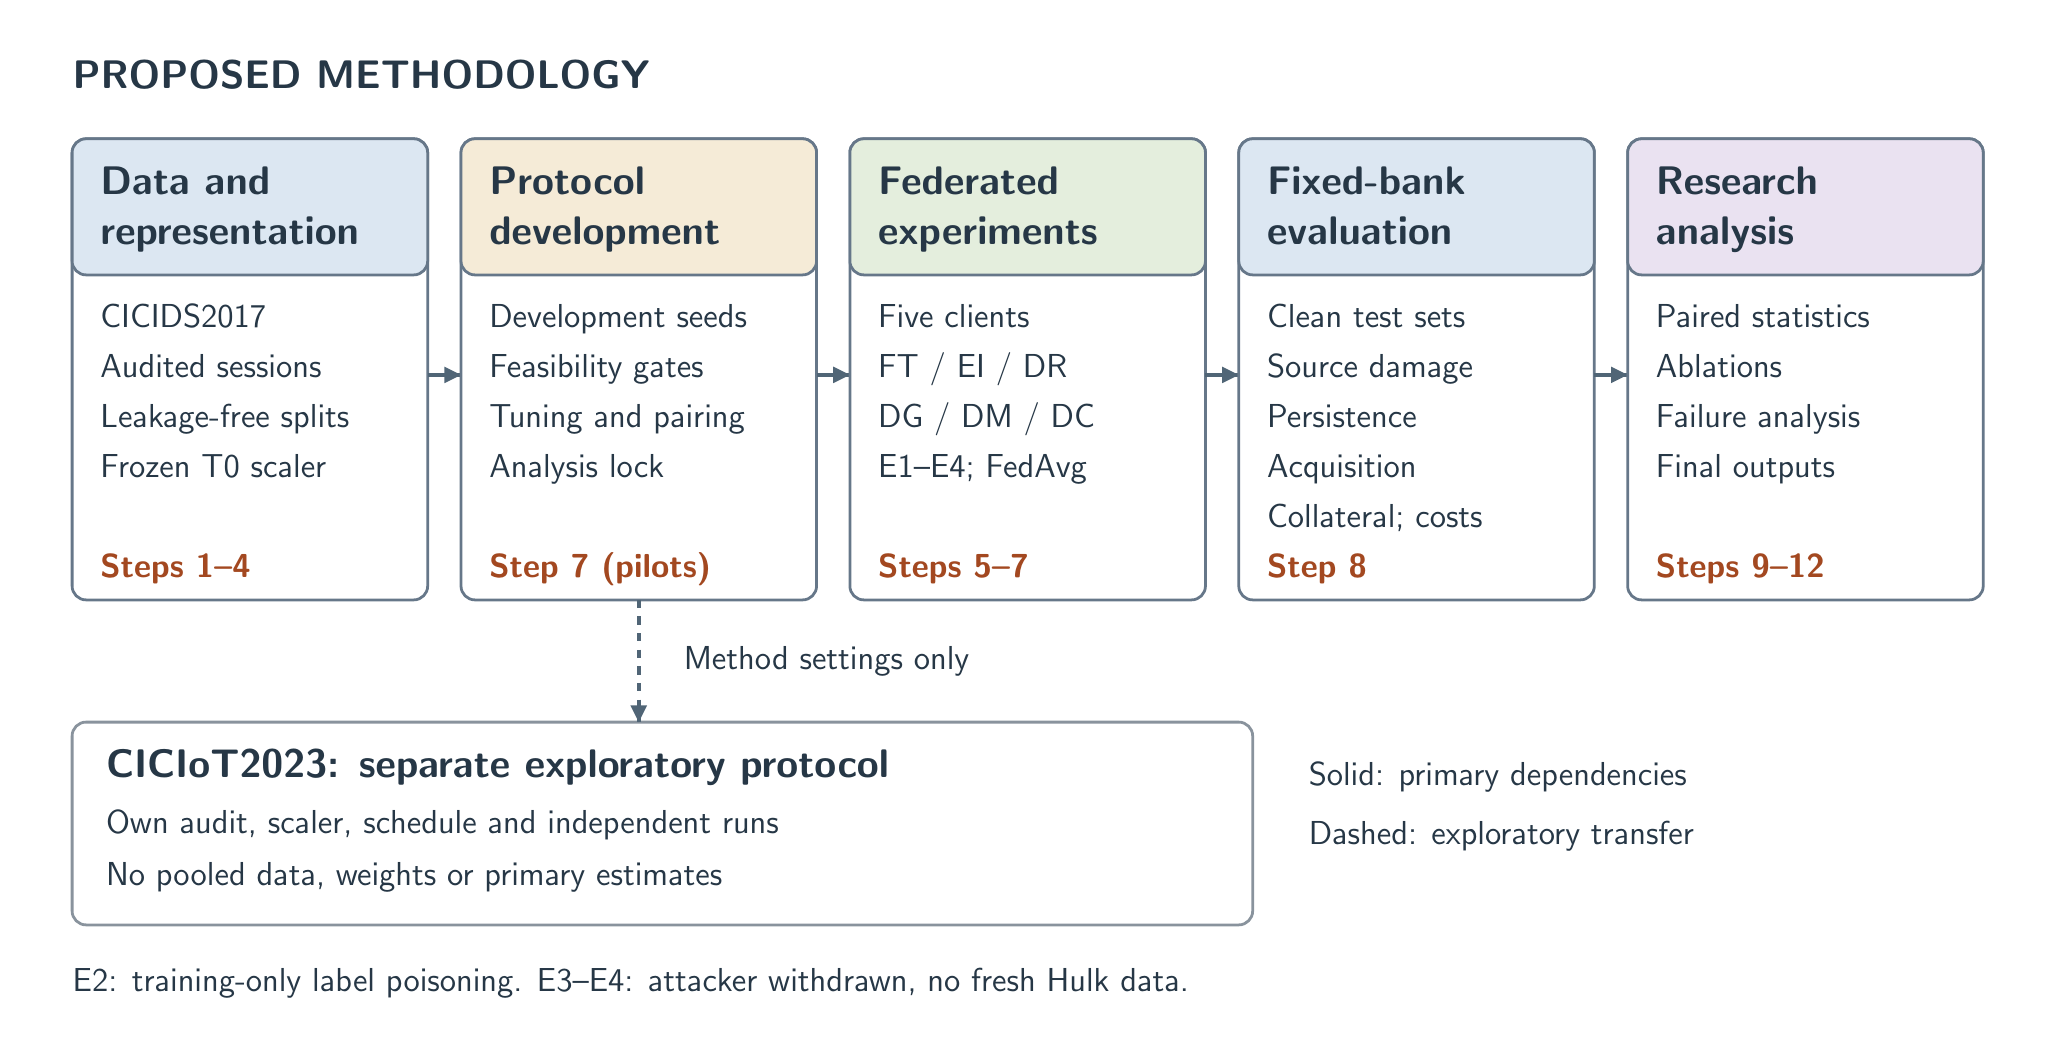
\begin{tikzpicture}[x=1bp,y=-1bp]
\path[use as bounding box] (0,0) rectangle (720,358);
\node[anchor=base west,inner sep=0,text={rgb,255:red,38;green,55;blue,70},font=\sffamily\bfseries\fontsize{15}{17.25}\selectfont] at (16,22) {PROPOSED METHODOLOGY};
\path[draw={rgb,255:red,102;green,119;blue,137},fill={rgb,255:red,255;green,255;blue,255},line width=1bp,rounded corners=5bp] (16,40) rectangle (144,206);
\path[draw={rgb,255:red,102;green,119;blue,137},fill={rgb,255:red,220;green,231;blue,242},line width=1bp,rounded corners=5bp] (16,40) rectangle (144,89);
\node[anchor=base west,inner sep=0,text={rgb,255:red,38;green,55;blue,70},font=\sffamily\bfseries\fontsize{15}{17.25}\selectfont] at (26,60) {Data and};
\node[anchor=base west,inner sep=0,text={rgb,255:red,38;green,55;blue,70},font=\sffamily\bfseries\fontsize{15}{17.25}\selectfont] at (26,78) {representation};
\node[anchor=base west,inner sep=0,text={rgb,255:red,38;green,55;blue,70},font=\sffamily\fontsize{12}{13.8}\selectfont] at (26,108) {CICIDS2017};
\node[anchor=base west,inner sep=0,text={rgb,255:red,38;green,55;blue,70},font=\sffamily\fontsize{12}{13.8}\selectfont] at (26,126) {Audited sessions};
\node[anchor=base west,inner sep=0,text={rgb,255:red,38;green,55;blue,70},font=\sffamily\fontsize{12}{13.8}\selectfont] at (26,144) {Leakage-free splits};
\node[anchor=base west,inner sep=0,text={rgb,255:red,38;green,55;blue,70},font=\sffamily\fontsize{12}{13.8}\selectfont] at (26,162) {Frozen T0 scaler};
\node[anchor=base west,inner sep=0,text={rgb,255:red,163;green,72;blue,32},font=\sffamily\bfseries\fontsize{12}{13.8}\selectfont] at (26,198) {Steps 1--4};
\path[draw={rgb,255:red,80;green,101;blue,118},line width=1.4bp] (144,125) -- (156,125);
\path[fill={rgb,255:red,80;green,101;blue,118}] (156.000,125.000) -- (150.000,122.000) -- (150.000,128.000) -- cycle;
\path[draw={rgb,255:red,102;green,119;blue,137},fill={rgb,255:red,255;green,255;blue,255},line width=1bp,rounded corners=5bp] (156,40) rectangle (284,206);
\path[draw={rgb,255:red,102;green,119;blue,137},fill={rgb,255:red,245;green,235;blue,215},line width=1bp,rounded corners=5bp] (156,40) rectangle (284,89);
\node[anchor=base west,inner sep=0,text={rgb,255:red,38;green,55;blue,70},font=\sffamily\bfseries\fontsize{15}{17.25}\selectfont] at (166,60) {Protocol};
\node[anchor=base west,inner sep=0,text={rgb,255:red,38;green,55;blue,70},font=\sffamily\bfseries\fontsize{15}{17.25}\selectfont] at (166,78) {development};
\node[anchor=base west,inner sep=0,text={rgb,255:red,38;green,55;blue,70},font=\sffamily\fontsize{12}{13.8}\selectfont] at (166,108) {Development seeds};
\node[anchor=base west,inner sep=0,text={rgb,255:red,38;green,55;blue,70},font=\sffamily\fontsize{12}{13.8}\selectfont] at (166,126) {Feasibility gates};
\node[anchor=base west,inner sep=0,text={rgb,255:red,38;green,55;blue,70},font=\sffamily\fontsize{12}{13.8}\selectfont] at (166,144) {Tuning and pairing};
\node[anchor=base west,inner sep=0,text={rgb,255:red,38;green,55;blue,70},font=\sffamily\fontsize{12}{13.8}\selectfont] at (166,162) {Analysis lock};
\node[anchor=base west,inner sep=0,text={rgb,255:red,163;green,72;blue,32},font=\sffamily\bfseries\fontsize{12}{13.8}\selectfont] at (166,198) {Step 7 (pilots)};
\path[draw={rgb,255:red,80;green,101;blue,118},line width=1.4bp] (284,125) -- (296,125);
\path[fill={rgb,255:red,80;green,101;blue,118}] (296.000,125.000) -- (290.000,122.000) -- (290.000,128.000) -- cycle;
\path[draw={rgb,255:red,102;green,119;blue,137},fill={rgb,255:red,255;green,255;blue,255},line width=1bp,rounded corners=5bp] (296,40) rectangle (424,206);
\path[draw={rgb,255:red,102;green,119;blue,137},fill={rgb,255:red,228;green,238;blue,221},line width=1bp,rounded corners=5bp] (296,40) rectangle (424,89);
\node[anchor=base west,inner sep=0,text={rgb,255:red,38;green,55;blue,70},font=\sffamily\bfseries\fontsize{15}{17.25}\selectfont] at (306,60) {Federated};
\node[anchor=base west,inner sep=0,text={rgb,255:red,38;green,55;blue,70},font=\sffamily\bfseries\fontsize{15}{17.25}\selectfont] at (306,78) {experiments};
\node[anchor=base west,inner sep=0,text={rgb,255:red,38;green,55;blue,70},font=\sffamily\fontsize{12}{13.8}\selectfont] at (306,108) {Five clients};
\node[anchor=base west,inner sep=0,text={rgb,255:red,38;green,55;blue,70},font=\sffamily\fontsize{12}{13.8}\selectfont] at (306,126) {FT / EI / DR};
\node[anchor=base west,inner sep=0,text={rgb,255:red,38;green,55;blue,70},font=\sffamily\fontsize{12}{13.8}\selectfont] at (306,144) {DG / DM / DC};
\node[anchor=base west,inner sep=0,text={rgb,255:red,38;green,55;blue,70},font=\sffamily\fontsize{12}{13.8}\selectfont] at (306,162) {E1--E4; FedAvg};
\node[anchor=base west,inner sep=0,text={rgb,255:red,163;green,72;blue,32},font=\sffamily\bfseries\fontsize{12}{13.8}\selectfont] at (306,198) {Steps 5--7};
\path[draw={rgb,255:red,80;green,101;blue,118},line width=1.4bp] (424,125) -- (436,125);
\path[fill={rgb,255:red,80;green,101;blue,118}] (436.000,125.000) -- (430.000,122.000) -- (430.000,128.000) -- cycle;
\path[draw={rgb,255:red,102;green,119;blue,137},fill={rgb,255:red,255;green,255;blue,255},line width=1bp,rounded corners=5bp] (436,40) rectangle (564,206);
\path[draw={rgb,255:red,102;green,119;blue,137},fill={rgb,255:red,220;green,231;blue,242},line width=1bp,rounded corners=5bp] (436,40) rectangle (564,89);
\node[anchor=base west,inner sep=0,text={rgb,255:red,38;green,55;blue,70},font=\sffamily\bfseries\fontsize{15}{17.25}\selectfont] at (446,60) {Fixed-bank};
\node[anchor=base west,inner sep=0,text={rgb,255:red,38;green,55;blue,70},font=\sffamily\bfseries\fontsize{15}{17.25}\selectfont] at (446,78) {evaluation};
\node[anchor=base west,inner sep=0,text={rgb,255:red,38;green,55;blue,70},font=\sffamily\fontsize{12}{13.8}\selectfont] at (446,108) {Clean test sets};
\node[anchor=base west,inner sep=0,text={rgb,255:red,38;green,55;blue,70},font=\sffamily\fontsize{12}{13.8}\selectfont] at (446,126) {Source damage};
\node[anchor=base west,inner sep=0,text={rgb,255:red,38;green,55;blue,70},font=\sffamily\fontsize{12}{13.8}\selectfont] at (446,144) {Persistence};
\node[anchor=base west,inner sep=0,text={rgb,255:red,38;green,55;blue,70},font=\sffamily\fontsize{12}{13.8}\selectfont] at (446,162) {Acquisition};
\node[anchor=base west,inner sep=0,text={rgb,255:red,38;green,55;blue,70},font=\sffamily\fontsize{12}{13.8}\selectfont] at (446,180) {Collateral; costs};
\node[anchor=base west,inner sep=0,text={rgb,255:red,163;green,72;blue,32},font=\sffamily\bfseries\fontsize{12}{13.8}\selectfont] at (446,198) {Step 8};
\path[draw={rgb,255:red,80;green,101;blue,118},line width=1.4bp] (564,125) -- (576,125);
\path[fill={rgb,255:red,80;green,101;blue,118}] (576.000,125.000) -- (570.000,122.000) -- (570.000,128.000) -- cycle;
\path[draw={rgb,255:red,102;green,119;blue,137},fill={rgb,255:red,255;green,255;blue,255},line width=1bp,rounded corners=5bp] (576,40) rectangle (704,206);
\path[draw={rgb,255:red,102;green,119;blue,137},fill={rgb,255:red,234;green,226;blue,241},line width=1bp,rounded corners=5bp] (576,40) rectangle (704,89);
\node[anchor=base west,inner sep=0,text={rgb,255:red,38;green,55;blue,70},font=\sffamily\bfseries\fontsize{15}{17.25}\selectfont] at (586,60) {Research};
\node[anchor=base west,inner sep=0,text={rgb,255:red,38;green,55;blue,70},font=\sffamily\bfseries\fontsize{15}{17.25}\selectfont] at (586,78) {analysis};
\node[anchor=base west,inner sep=0,text={rgb,255:red,38;green,55;blue,70},font=\sffamily\fontsize{12}{13.8}\selectfont] at (586,108) {Paired statistics};
\node[anchor=base west,inner sep=0,text={rgb,255:red,38;green,55;blue,70},font=\sffamily\fontsize{12}{13.8}\selectfont] at (586,126) {Ablations};
\node[anchor=base west,inner sep=0,text={rgb,255:red,38;green,55;blue,70},font=\sffamily\fontsize{12}{13.8}\selectfont] at (586,144) {Failure analysis};
\node[anchor=base west,inner sep=0,text={rgb,255:red,38;green,55;blue,70},font=\sffamily\fontsize{12}{13.8}\selectfont] at (586,162) {Final outputs};
\node[anchor=base west,inner sep=0,text={rgb,255:red,163;green,72;blue,32},font=\sffamily\bfseries\fontsize{12}{13.8}\selectfont] at (586,198) {Steps 9--12};
\path[draw={rgb,255:red,137;green,147;blue,157},fill={rgb,255:red,255;green,255;blue,255},line width=1bp,rounded corners=5bp] (16,250) rectangle (441,323);
\node[anchor=base west,inner sep=0,text={rgb,255:red,38;green,55;blue,70},font=\sffamily\bfseries\fontsize{15}{17.25}\selectfont] at (28,270) {CICIoT2023: separate exploratory protocol};
\node[anchor=base west,inner sep=0,text={rgb,255:red,38;green,55;blue,70},font=\sffamily\fontsize{12}{13.8}\selectfont] at (28,290) {Own audit, scaler, schedule and independent runs};
\node[anchor=base west,inner sep=0,text={rgb,255:red,38;green,55;blue,70},font=\sffamily\fontsize{12}{13.8}\selectfont] at (28,309) {No pooled data, weights or primary estimates};
\path[draw={rgb,255:red,80;green,101;blue,118},line width=1.4bp,dashed] (220,206) -- (220,250);
\path[fill={rgb,255:red,80;green,101;blue,118}] (220.000,250.000) -- (223.000,244.000) -- (217.000,244.000) -- cycle;
\node[anchor=base west,inner sep=0,text={rgb,255:red,38;green,55;blue,70},font=\sffamily\fontsize{12}{13.8}\selectfont] at (236,231) {Method settings only};
\node[anchor=base west,inner sep=0,text={rgb,255:red,38;green,55;blue,70},font=\sffamily\fontsize{12}{13.8}\selectfont] at (461,273) {Solid: primary dependencies};
\node[anchor=base west,inner sep=0,text={rgb,255:red,38;green,55;blue,70},font=\sffamily\fontsize{12}{13.8}\selectfont] at (461,294) {Dashed: exploratory transfer};
\node[anchor=base west,inner sep=0,text={rgb,255:red,38;green,55;blue,70},font=\sffamily\fontsize{12}{13.8}\selectfont] at (16,347) {E2: training-only label poisoning. E3--E4: attacker withdrawn, no fresh Hulk data.};
\end{tikzpicture}
}
\caption{Methodology overview. The orange labels show which of the twelve methodology steps each phase covers. Solid arrows pass audited data, locked settings, trained models and predictions forward; the dashed branch transfers only method settings to the separate exploratory CICIoT2023 study.}
\label{fig:methodology}
\end{figure}

\begin{figure}[htbp]
\centering
\resizebox{\linewidth}{!}{%
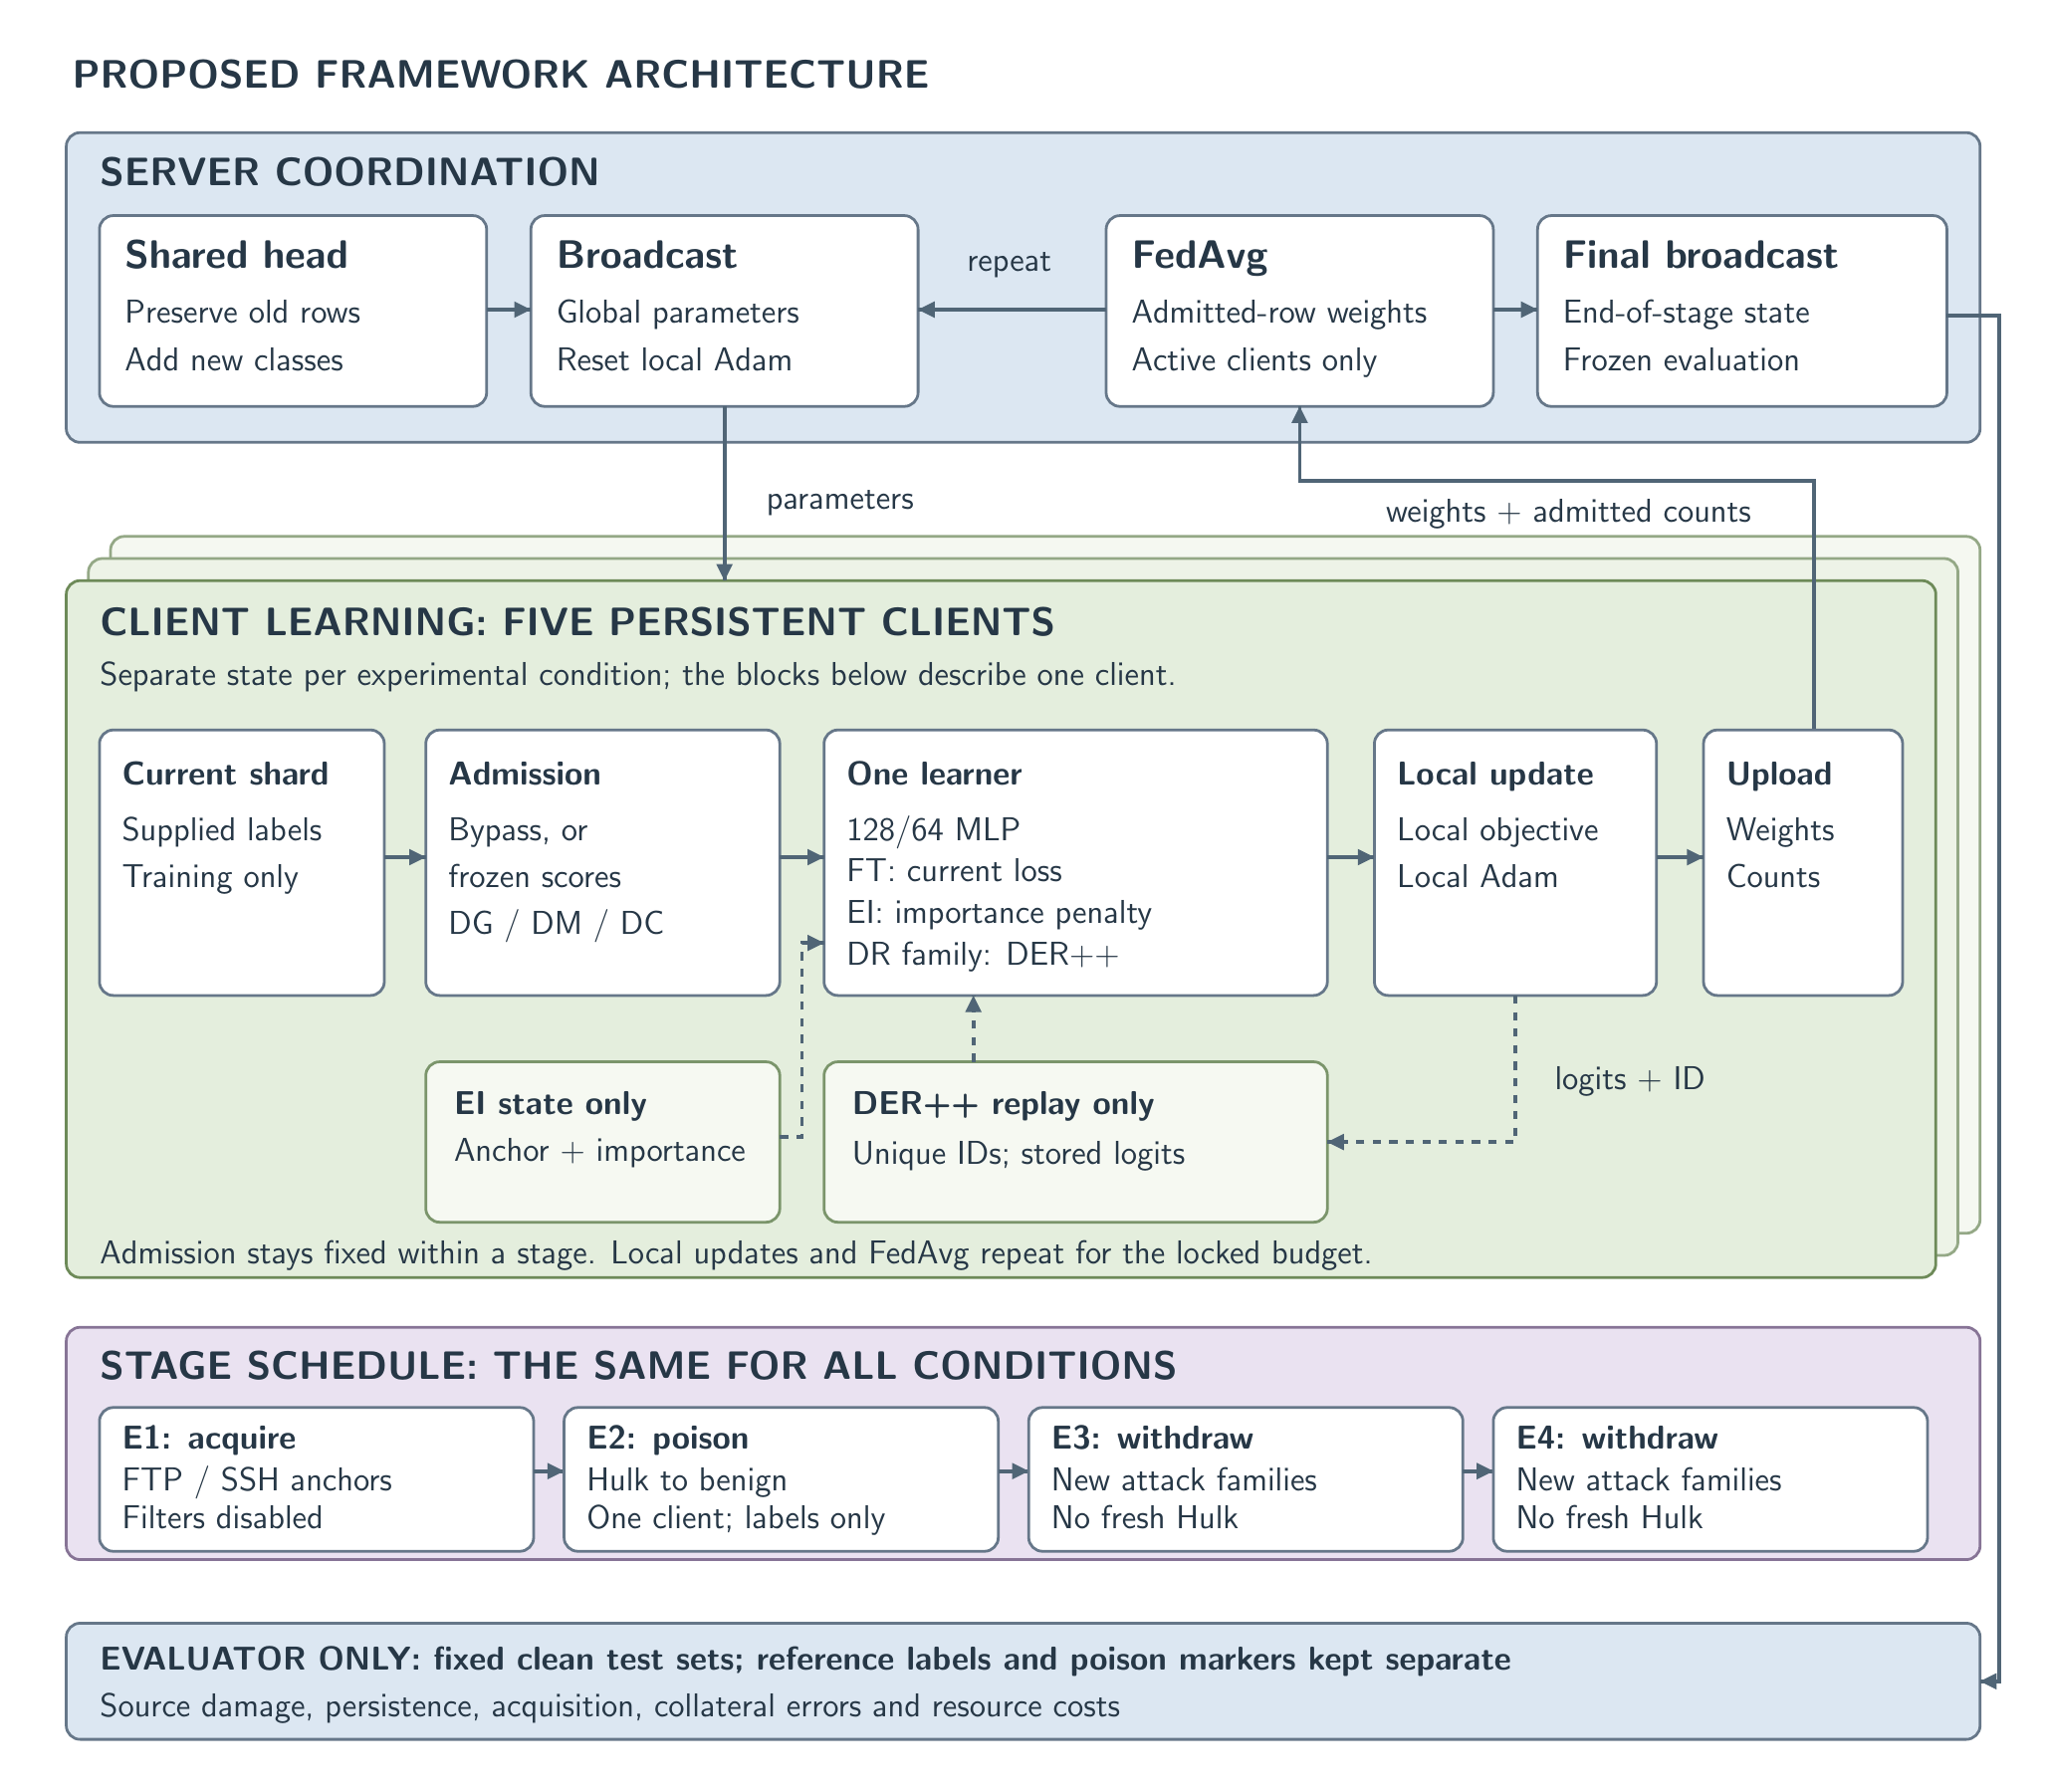
\begin{tikzpicture}[x=1bp,y=-1bp]
\path[use as bounding box] (0,0) rectangle (720,628);
\node[anchor=base west,inner sep=0,text={rgb,255:red,38;green,55;blue,70},font=\sffamily\bfseries\fontsize{15}{17.25}\selectfont] at (16,22) {PROPOSED FRAMEWORK ARCHITECTURE};
\path[draw={rgb,255:red,102;green,119;blue,137},fill={rgb,255:red,220;green,231;blue,242},line width=1bp,rounded corners=5bp] (14,38) rectangle (706,150);
\node[anchor=base west,inner sep=0,text={rgb,255:red,38;green,55;blue,70},font=\sffamily\bfseries\fontsize{15}{17.25}\selectfont] at (26,57) {SERVER COORDINATION};
\path[draw={rgb,255:red,102;green,119;blue,137},fill={rgb,255:red,255;green,255;blue,255},line width=1bp,rounded corners=5bp] (26,68) rectangle (166,137);
\node[anchor=base west,inner sep=0,text={rgb,255:red,38;green,55;blue,70},font=\sffamily\bfseries\fontsize{14}{16.1}\selectfont] at (35,87) {Shared head};
\node[anchor=base west,inner sep=0,text={rgb,255:red,38;green,55;blue,70},font=\sffamily\fontsize{12}{13.8}\selectfont] at (35,107) {Preserve old rows};
\node[anchor=base west,inner sep=0,text={rgb,255:red,38;green,55;blue,70},font=\sffamily\fontsize{12}{13.8}\selectfont] at (35,124) {Add new classes};
\path[draw={rgb,255:red,102;green,119;blue,137},fill={rgb,255:red,255;green,255;blue,255},line width=1bp,rounded corners=5bp] (182,68) rectangle (322,137);
\node[anchor=base west,inner sep=0,text={rgb,255:red,38;green,55;blue,70},font=\sffamily\bfseries\fontsize{14}{16.1}\selectfont] at (191,87) {Broadcast};
\node[anchor=base west,inner sep=0,text={rgb,255:red,38;green,55;blue,70},font=\sffamily\fontsize{12}{13.8}\selectfont] at (191,107) {Global parameters};
\node[anchor=base west,inner sep=0,text={rgb,255:red,38;green,55;blue,70},font=\sffamily\fontsize{12}{13.8}\selectfont] at (191,124) {Reset local Adam};
\path[draw={rgb,255:red,102;green,119;blue,137},fill={rgb,255:red,255;green,255;blue,255},line width=1bp,rounded corners=5bp] (390,68) rectangle (530,137);
\node[anchor=base west,inner sep=0,text={rgb,255:red,38;green,55;blue,70},font=\sffamily\bfseries\fontsize{14}{16.1}\selectfont] at (399,87) {FedAvg};
\node[anchor=base west,inner sep=0,text={rgb,255:red,38;green,55;blue,70},font=\sffamily\fontsize{12}{13.8}\selectfont] at (399,107) {Admitted-row weights};
\node[anchor=base west,inner sep=0,text={rgb,255:red,38;green,55;blue,70},font=\sffamily\fontsize{12}{13.8}\selectfont] at (399,124) {Active clients only};
\path[draw={rgb,255:red,102;green,119;blue,137},fill={rgb,255:red,255;green,255;blue,255},line width=1bp,rounded corners=5bp] (546,68) rectangle (694,137);
\node[anchor=base west,inner sep=0,text={rgb,255:red,38;green,55;blue,70},font=\sffamily\bfseries\fontsize{14}{16.1}\selectfont] at (555,87) {Final broadcast};
\node[anchor=base west,inner sep=0,text={rgb,255:red,38;green,55;blue,70},font=\sffamily\fontsize{12}{13.8}\selectfont] at (555,107) {End-of-stage state};
\node[anchor=base west,inner sep=0,text={rgb,255:red,38;green,55;blue,70},font=\sffamily\fontsize{12}{13.8}\selectfont] at (555,124) {Frozen evaluation};
\path[draw={rgb,255:red,80;green,101;blue,118},line width=1.4bp] (166,102) -- (182,102);
\path[fill={rgb,255:red,80;green,101;blue,118}] (182.000,102.000) -- (176.000,99.000) -- (176.000,105.000) -- cycle;
\path[draw={rgb,255:red,80;green,101;blue,118},line width=1.4bp] (530,102) -- (546,102);
\path[fill={rgb,255:red,80;green,101;blue,118}] (546.000,102.000) -- (540.000,99.000) -- (540.000,105.000) -- cycle;
\path[draw={rgb,255:red,80;green,101;blue,118},line width=1.4bp] (390,102) -- (322,102);
\path[fill={rgb,255:red,80;green,101;blue,118}] (322.000,102.000) -- (328.000,105.000) -- (328.000,99.000) -- cycle;
\node[anchor=base,inner sep=0,text={rgb,255:red,38;green,55;blue,70},font=\sffamily\fontsize{12}{13.8}\selectfont] at (355,88) {repeat};
\path[draw={rgb,255:red,148;green,168;blue,134},fill={rgb,255:red,245;green,248;blue,241},line width=1bp,rounded corners=5bp] (30,184) rectangle (706,436);
\path[draw={rgb,255:red,148;green,168;blue,134},fill={rgb,255:red,237;green,243;blue,231},line width=1bp,rounded corners=5bp] (22,192) rectangle (698,444);
\path[draw={rgb,255:red,109;green,138;blue,88},fill={rgb,255:red,228;green,238;blue,221},line width=1bp,rounded corners=5bp] (14,200) rectangle (690,452);
\node[anchor=base west,inner sep=0,text={rgb,255:red,38;green,55;blue,70},font=\sffamily\bfseries\fontsize{15}{17.25}\selectfont] at (26,220) {CLIENT LEARNING: FIVE PERSISTENT CLIENTS};
\node[anchor=base west,inner sep=0,text={rgb,255:red,38;green,55;blue,70},font=\sffamily\fontsize{12}{13.8}\selectfont] at (26,238) {Separate state per experimental condition; the blocks below describe one client.};
\path[draw={rgb,255:red,80;green,101;blue,118},line width=1.4bp] (252,137) -- (252,200);
\path[fill={rgb,255:red,80;green,101;blue,118}] (252.000,200.000) -- (255.000,194.000) -- (249.000,194.000) -- cycle;
\node[anchor=base west,inner sep=0,text={rgb,255:red,38;green,55;blue,70},font=\sffamily\fontsize{12}{13.8}\selectfont] at (267,174) {parameters};
\path[draw={rgb,255:red,80;green,101;blue,118},line width=1.4bp] (646,254) -- (646,164) -- (460,164) -- (460,137);
\path[fill={rgb,255:red,80;green,101;blue,118}] (460.000,137.000) -- (457.000,143.000) -- (463.000,143.000) -- cycle;
\node[anchor=base west,inner sep=0,text={rgb,255:red,38;green,55;blue,70},font=\sffamily\fontsize{12}{13.8}\selectfont] at (491,179) {weights + admitted counts};
\path[draw={rgb,255:red,102;green,119;blue,137},fill={rgb,255:red,255;green,255;blue,255},line width=1bp,rounded corners=5bp] (26,254) rectangle (129,350);
\node[anchor=base west,inner sep=0,text={rgb,255:red,38;green,55;blue,70},font=\sffamily\bfseries\fontsize{13}{14.95}\selectfont] at (34,274) {Current shard};
\node[anchor=base west,inner sep=0,text={rgb,255:red,38;green,55;blue,70},font=\sffamily\fontsize{12}{13.8}\selectfont] at (34,294) {Supplied labels};
\node[anchor=base west,inner sep=0,text={rgb,255:red,38;green,55;blue,70},font=\sffamily\fontsize{12}{13.8}\selectfont] at (34,311) {Training only};
\path[draw={rgb,255:red,102;green,119;blue,137},fill={rgb,255:red,255;green,255;blue,255},line width=1bp,rounded corners=5bp] (144,254) rectangle (272,350);
\node[anchor=base west,inner sep=0,text={rgb,255:red,38;green,55;blue,70},font=\sffamily\bfseries\fontsize{13}{14.95}\selectfont] at (152,274) {Admission};
\node[anchor=base west,inner sep=0,text={rgb,255:red,38;green,55;blue,70},font=\sffamily\fontsize{12}{13.8}\selectfont] at (152,294) {Bypass, or};
\node[anchor=base west,inner sep=0,text={rgb,255:red,38;green,55;blue,70},font=\sffamily\fontsize{12}{13.8}\selectfont] at (152,311) {frozen scores};
\node[anchor=base west,inner sep=0,text={rgb,255:red,38;green,55;blue,70},font=\sffamily\fontsize{12}{13.8}\selectfont] at (152,328) {DG / DM / DC};
\path[draw={rgb,255:red,102;green,119;blue,137},fill={rgb,255:red,255;green,255;blue,255},line width=1bp,rounded corners=5bp] (288,254) rectangle (470,350);
\node[anchor=base west,inner sep=0,text={rgb,255:red,38;green,55;blue,70},font=\sffamily\bfseries\fontsize{13}{14.95}\selectfont] at (296,274) {One learner};
\node[anchor=base west,inner sep=0,text={rgb,255:red,38;green,55;blue,70},font=\sffamily\fontsize{12}{13.8}\selectfont] at (296,294) {128/64 MLP};
\node[anchor=base west,inner sep=0,text={rgb,255:red,38;green,55;blue,70},font=\sffamily\fontsize{12}{13.8}\selectfont] at (296,309) {FT: current loss};
\node[anchor=base west,inner sep=0,text={rgb,255:red,38;green,55;blue,70},font=\sffamily\fontsize{12}{13.8}\selectfont] at (296,324) {EI: importance penalty};
\node[anchor=base west,inner sep=0,text={rgb,255:red,38;green,55;blue,70},font=\sffamily\fontsize{12}{13.8}\selectfont] at (296,339) {DR family: DER++};
\path[draw={rgb,255:red,102;green,119;blue,137},fill={rgb,255:red,255;green,255;blue,255},line width=1bp,rounded corners=5bp] (487,254) rectangle (589,350);
\node[anchor=base west,inner sep=0,text={rgb,255:red,38;green,55;blue,70},font=\sffamily\bfseries\fontsize{13}{14.95}\selectfont] at (495,274) {Local update};
\node[anchor=base west,inner sep=0,text={rgb,255:red,38;green,55;blue,70},font=\sffamily\fontsize{12}{13.8}\selectfont] at (495,294) {Local objective};
\node[anchor=base west,inner sep=0,text={rgb,255:red,38;green,55;blue,70},font=\sffamily\fontsize{12}{13.8}\selectfont] at (495,311) {Local Adam};
\path[draw={rgb,255:red,102;green,119;blue,137},fill={rgb,255:red,255;green,255;blue,255},line width=1bp,rounded corners=5bp] (606,254) rectangle (678,350);
\node[anchor=base west,inner sep=0,text={rgb,255:red,38;green,55;blue,70},font=\sffamily\bfseries\fontsize{13}{14.95}\selectfont] at (614,274) {Upload};
\node[anchor=base west,inner sep=0,text={rgb,255:red,38;green,55;blue,70},font=\sffamily\fontsize{12}{13.8}\selectfont] at (614,294) {Weights};
\node[anchor=base west,inner sep=0,text={rgb,255:red,38;green,55;blue,70},font=\sffamily\fontsize{12}{13.8}\selectfont] at (614,311) {Counts};
\path[draw={rgb,255:red,80;green,101;blue,118},line width=1.4bp] (129,300) -- (144,300);
\path[fill={rgb,255:red,80;green,101;blue,118}] (144.000,300.000) -- (138.000,297.000) -- (138.000,303.000) -- cycle;
\path[draw={rgb,255:red,80;green,101;blue,118},line width=1.4bp] (272,300) -- (288,300);
\path[fill={rgb,255:red,80;green,101;blue,118}] (288.000,300.000) -- (282.000,297.000) -- (282.000,303.000) -- cycle;
\path[draw={rgb,255:red,80;green,101;blue,118},line width=1.4bp] (470,300) -- (487,300);
\path[fill={rgb,255:red,80;green,101;blue,118}] (487.000,300.000) -- (481.000,297.000) -- (481.000,303.000) -- cycle;
\path[draw={rgb,255:red,80;green,101;blue,118},line width=1.4bp] (589,300) -- (606,300);
\path[fill={rgb,255:red,80;green,101;blue,118}] (606.000,300.000) -- (600.000,297.000) -- (600.000,303.000) -- cycle;
\path[draw={rgb,255:red,123;green,149;blue,107},fill={rgb,255:red,246;green,249;blue,242},line width=1bp,rounded corners=5bp] (144,374) rectangle (272,432);
\node[anchor=base west,inner sep=0,text={rgb,255:red,38;green,55;blue,70},font=\sffamily\bfseries\fontsize{13}{14.95}\selectfont] at (154,393) {EI state only};
\node[anchor=base west,inner sep=0,text={rgb,255:red,38;green,55;blue,70},font=\sffamily\fontsize{12}{13.8}\selectfont] at (154,410) {Anchor + importance};
\path[draw={rgb,255:red,80;green,101;blue,118},line width=1.4bp,dashed] (272,401) -- (280,401) -- (280,331) -- (288,331);
\path[fill={rgb,255:red,80;green,101;blue,118}] (288.000,331.000) -- (282.000,328.000) -- (282.000,334.000) -- cycle;
\path[draw={rgb,255:red,123;green,149;blue,107},fill={rgb,255:red,246;green,249;blue,242},line width=1bp,rounded corners=5bp] (288,374) rectangle (470,432);
\node[anchor=base west,inner sep=0,text={rgb,255:red,38;green,55;blue,70},font=\sffamily\bfseries\fontsize{13}{14.95}\selectfont] at (298,393) {DER++ replay only};
\node[anchor=base west,inner sep=0,text={rgb,255:red,38;green,55;blue,70},font=\sffamily\fontsize{12}{13.8}\selectfont] at (298,411) {Unique IDs; stored logits};
\path[draw={rgb,255:red,80;green,101;blue,118},line width=1.4bp,dashed] (342,374) -- (342,350);
\path[fill={rgb,255:red,80;green,101;blue,118}] (342.000,350.000) -- (339.000,356.000) -- (345.000,356.000) -- cycle;
\path[draw={rgb,255:red,80;green,101;blue,118},line width=1.4bp,dashed] (538,350) -- (538,403) -- (470,403);
\path[fill={rgb,255:red,80;green,101;blue,118}] (470.000,403.000) -- (476.000,406.000) -- (476.000,400.000) -- cycle;
\node[anchor=base west,inner sep=0,text={rgb,255:red,38;green,55;blue,70},font=\sffamily\fontsize{12}{13.8}\selectfont] at (552,384) {logits + ID};
\node[anchor=base west,inner sep=0,text={rgb,255:red,38;green,55;blue,70},font=\sffamily\fontsize{12}{13.8}\selectfont] at (26,447) {Admission stays fixed within a stage. Local updates and FedAvg repeat for the locked budget.};
\path[draw={rgb,255:red,135;green,116;blue,150},fill={rgb,255:red,234;green,226;blue,241},line width=1bp,rounded corners=5bp] (14,470) rectangle (706,554);
\node[anchor=base west,inner sep=0,text={rgb,255:red,38;green,55;blue,70},font=\sffamily\bfseries\fontsize{15}{17.25}\selectfont] at (26,489) {STAGE SCHEDULE: THE SAME FOR ALL CONDITIONS};
\path[draw={rgb,255:red,102;green,119;blue,137},fill={rgb,255:red,255;green,255;blue,255},line width=1bp,rounded corners=5bp] (26,499) rectangle (183,551);
\node[anchor=base west,inner sep=0,text={rgb,255:red,38;green,55;blue,70},font=\sffamily\bfseries\fontsize{13}{14.95}\selectfont] at (34,514) {E1: acquire};
\node[anchor=base west,inner sep=0,text={rgb,255:red,38;green,55;blue,70},font=\sffamily\fontsize{12}{13.8}\selectfont] at (34,529) {FTP / SSH anchors};
\node[anchor=base west,inner sep=0,text={rgb,255:red,38;green,55;blue,70},font=\sffamily\fontsize{12}{13.8}\selectfont] at (34,543) {Filters disabled};
\path[draw={rgb,255:red,80;green,101;blue,118},line width=1.4bp] (183,522) -- (194,522);
\path[fill={rgb,255:red,80;green,101;blue,118}] (194.000,522.000) -- (188.000,519.000) -- (188.000,525.000) -- cycle;
\path[draw={rgb,255:red,102;green,119;blue,137},fill={rgb,255:red,255;green,255;blue,255},line width=1bp,rounded corners=5bp] (194,499) rectangle (351,551);
\node[anchor=base west,inner sep=0,text={rgb,255:red,38;green,55;blue,70},font=\sffamily\bfseries\fontsize{13}{14.95}\selectfont] at (202,514) {E2: poison};
\node[anchor=base west,inner sep=0,text={rgb,255:red,38;green,55;blue,70},font=\sffamily\fontsize{12}{13.8}\selectfont] at (202,529) {Hulk to benign};
\node[anchor=base west,inner sep=0,text={rgb,255:red,38;green,55;blue,70},font=\sffamily\fontsize{12}{13.8}\selectfont] at (202,543) {One client; labels only};
\path[draw={rgb,255:red,80;green,101;blue,118},line width=1.4bp] (351,522) -- (362,522);
\path[fill={rgb,255:red,80;green,101;blue,118}] (362.000,522.000) -- (356.000,519.000) -- (356.000,525.000) -- cycle;
\path[draw={rgb,255:red,102;green,119;blue,137},fill={rgb,255:red,255;green,255;blue,255},line width=1bp,rounded corners=5bp] (362,499) rectangle (519,551);
\node[anchor=base west,inner sep=0,text={rgb,255:red,38;green,55;blue,70},font=\sffamily\bfseries\fontsize{13}{14.95}\selectfont] at (370,514) {E3: withdraw};
\node[anchor=base west,inner sep=0,text={rgb,255:red,38;green,55;blue,70},font=\sffamily\fontsize{12}{13.8}\selectfont] at (370,529) {New attack families};
\node[anchor=base west,inner sep=0,text={rgb,255:red,38;green,55;blue,70},font=\sffamily\fontsize{12}{13.8}\selectfont] at (370,543) {No fresh Hulk};
\path[draw={rgb,255:red,80;green,101;blue,118},line width=1.4bp] (519,522) -- (530,522);
\path[fill={rgb,255:red,80;green,101;blue,118}] (530.000,522.000) -- (524.000,519.000) -- (524.000,525.000) -- cycle;
\path[draw={rgb,255:red,102;green,119;blue,137},fill={rgb,255:red,255;green,255;blue,255},line width=1bp,rounded corners=5bp] (530,499) rectangle (687,551);
\node[anchor=base west,inner sep=0,text={rgb,255:red,38;green,55;blue,70},font=\sffamily\bfseries\fontsize{13}{14.95}\selectfont] at (538,514) {E4: withdraw};
\node[anchor=base west,inner sep=0,text={rgb,255:red,38;green,55;blue,70},font=\sffamily\fontsize{12}{13.8}\selectfont] at (538,529) {New attack families};
\node[anchor=base west,inner sep=0,text={rgb,255:red,38;green,55;blue,70},font=\sffamily\fontsize{12}{13.8}\selectfont] at (538,543) {No fresh Hulk};
\path[draw={rgb,255:red,102;green,119;blue,137},fill={rgb,255:red,220;green,231;blue,242},line width=1bp,rounded corners=5bp] (14,577) rectangle (706,619);
\node[anchor=base west,inner sep=0,text={rgb,255:red,38;green,55;blue,70},font=\sffamily\bfseries\fontsize{13}{14.95}\selectfont] at (26,594) {EVALUATOR ONLY: fixed clean test sets; reference labels and poison markers kept separate};
\node[anchor=base west,inner sep=0,text={rgb,255:red,38;green,55;blue,70},font=\sffamily\fontsize{12}{13.8}\selectfont] at (26,611) {Source damage, persistence, acquisition, collateral errors and resource costs};
\path[draw={rgb,255:red,80;green,101;blue,118},line width=1.4bp] (694,104) -- (713,104) -- (713,598) -- (706,598);
\path[fill={rgb,255:red,80;green,101;blue,118}] (706.000,598.000) -- (712.000,601.000) -- (712.000,595.000) -- cycle;
\end{tikzpicture}
}
\caption{Proposed framework architecture. Server coordination and client learning repeat within each stage. FT/EI/DR are alternative learners; DG/DM/DC are alternative admission rules on DER++. Only EI keeps importance state and only DER++ conditions keep replay memory (dashed links). E2 corrupts training labels at one client only; E3--E4 contain no poison and no fresh Hulk data. The evaluator never influences training or admission.}
\label{fig:framework}
\end{figure}

%=====================================================================
\section{Scope and Threats to Validity}
\textbf{Internal validity.} Session reconstruction errors, known label defects in CICIDS2017, duplicate flows and shared optimiser settings could bias comparisons; the isolation rules, support floors and pilot gates are designed to catch them before final runs. The admission rule may still keep low-loss poisoned rows; this is a possible finding, not a flaw.

\textbf{External validity.} Clients are simulated by splitting one historical capture, so they do not represent independent organisations (a limitation shared with P5, P7 and P11). CICIoT2023 provides a separate check, and CPU timings and update sizes do not measure energy or network delay on real edge devices.

\textbf{Construct validity.} Source recall, persistent error, acquisition and anchor scores measure different things and are reported separately. The attacker controls labels only; a fully compromised client that skips filtering is a stronger, separate threat.

\textbf{Conclusion validity.} Twelve seeds measure training variability with fixed test sets, not variability between captures. Signed-rank tests assume roughly symmetric differences, and the two hypothesis families each control error at 5\%, not jointly.

%=====================================================================
\appendix
\section{Notation and Data-Isolation Conditions}
\label{app:notation}
\begin{table}[htbp]
\centering\footnotesize
\caption{Main notation.}
\label{tab:notation}
\begin{tabularx}{\linewidth}{L{4.6cm}Y}
\toprule
Symbol & Meaning\\
\midrule
$k,\ t,\ c,\ i,\ s$ & Client, stage, class, record and seed indices\\
$x_i,\ \widetilde y_i,\ y_i,\ \widehat y_i$ & Features; supplied (possibly poisoned), reference and predicted labels\\
$u_i,\ \sigma_i,\ \tau_i$ & Immutable record ID, session ID and timestamp (metadata only)\\
$\mathcal C_t,\ \mathcal C_t^{\rm new},\ C_t,\ \mathcal E_t$ & Classes seen so far, new classes at stage $t$, their number, scheduled new families\\
$W,\ b,\ \theta,\ f_{\theta,t}$ & Weights, biases, all parameters, output logits\\
$\mathcal B,\ m,\ z_i,\ \omega_i,\ S_i$ & Replay memory, its capacity (500), stored logits, their width, logit selector\\
$\lambda_E,\ \lambda_z,\ \lambda_y,\ I_a$ & Loss weights and accumulated parameter importance\\
$n_{k,c,t},\ K_{k,c,t}$ & Rows of class $c$ at client $k$ in stage $t$; admitted quota\\
$\rho,\ Q_{k,2}$ & Poison dose and number of flipped Hulk rows\\
$\mathcal S_{\rm tr/dev/te},\ \mathcal G_{\rm tr/dev/te},\ H_{\rm sha},\ \Psi_0$ & Splits, their sessions, content hash, frozen T0 scaler\\
$\mathrm{ASR},\ H,\ \Delta_{\rm rec},\ A,\ \mathrm{FAR}_B$ & Attack success, persistence, recall change, acquisition, benign false alarms\\
\bottomrule
\end{tabularx}
\end{table}
The splits must not share content or sessions, and the scaler is fitted on T0 only:
\begin{equation}
H_{\rm sha}(\mathcal S_{\rm tr})\cap H_{\rm sha}(\mathcal S_{\rm dev}\cup\mathcal S_{\rm te})=\varnothing,\quad
H_{\rm sha}(\mathcal S_{\rm dev})\cap H_{\rm sha}(\mathcal S_{\rm te})=\varnothing,\quad
\mathcal G_{\rm tr}\cap\mathcal G_{\rm dev}=\mathcal G_{\rm tr}\cap\mathcal G_{\rm te}=\mathcal G_{\rm dev}\cap\mathcal G_{\rm te}=\varnothing,
\label{eq:isolation}
\end{equation}
with $\Psi_0=\operatorname{FitMinMax}(\text{isolated T0 benign inputs})$. The same conditions hold between T0 and every supervised split.

\section{Statistical Details}
\label{app:stats}
For endpoint $U$, seed $s$ and learners $\mathsf A,\mathsf B$, the learner interaction is
\begin{equation}
\mathcal J_s^{\mathsf A,\mathsf B}(\rho;U)=[U_s^{\mathsf A,\rho}-U_s^{\mathsf A,0}]-[U_s^{\mathsf B,\rho}-U_s^{\mathsf B,0}],
\label{eq:interaction}
\end{equation}
and $\bar\delta=\frac1n\sum_s\delta_s$ is the mean paired difference over $n=12$ seeds. Wilcoxon signed-rank tests drop zero differences and average tied ranks \cite{wilcoxon}; Holm's procedure compares the $h$-th smallest p-value with $0.05/(L-h+1)$ within each family of $L$ tests \cite{holm}. Bootstrap intervals resample whole seeds 10,000 times:
\begin{equation}
\delta_b^*=\tfrac1n\sum_{\kappa=1}^n\delta_{\mathcal I_\kappa},\quad\mathcal I_\kappa\sim\operatorname{Uniform}\{1,\ldots,n\},\qquad
\mathrm{CI}_{\rm boot}=[\operatorname{Quant}_{0.025}(\delta^*),\operatorname{Quant}_{0.975}(\delta^*)].
\label{eq:bootstrap}
\end{equation}
Because twelve seeds give uncertain percentile coverage, a supplementary exact sign-flip interval $\{\delta_0:\mathfrak p_{\delta_0}>0.05\}$ is also reported, with
$\mathfrak p_{\delta_0}=2^{-n}\sum_{\varepsilon\in\{\pm1\}^n}\mathbf 1\{|\frac1n\sum_s\varepsilon_s(\delta_s-\delta_0)|\ge|\bar\delta-\delta_0|\}$.
\textbf{Resolution.} With twelve non-zero pairs the smallest possible two-sided p-value is $2/2^{12}\approx0.00049$. The strictest Holm thresholds are $0.05/18\approx0.0028$ (C1) and $0.05/11\approx0.0045$ (C2), so at least ten (C1) or nine (C2) non-zero pairs are needed for any rejection. These are resolution limits, not power estimates; failed runs are re-run as complete pairs, never imputed.

\section{CICIDS2017 Source Files}
\label{app:files}
Session metadata come from the eight matching TrafficLabelling CSVs in \emph{GeneratedLabelledFlows}. The eight MachineLearningCSV files are: \path{Monday-WorkingHours.pcap_ISCX.csv}, \path{Tuesday-WorkingHours.pcap_ISCX.csv}, \path{Wednesday-workingHours.pcap_ISCX.csv}, \path{Thursday-WorkingHours-Morning-WebAttacks.pcap_ISCX.csv}, \path{Thursday-WorkingHours-Afternoon-Infilteration.pcap_ISCX.csv}, \path{Friday-WorkingHours-Morning.pcap_ISCX.csv}, \path{Friday-WorkingHours-Afternoon-PortScan.pcap_ISCX.csv} and \path{Friday-WorkingHours-Afternoon-DDos.pcap_ISCX.csv}.

%=====================================================================
\begin{thebibliography}{99}
\bibitem{phase1} Saneedullah and A. Bilal, \enquote{Continual learning for network security: Phase 1 literature review and research gap identification,} Computer Networks course report, FAST-NUCES, 2026.
\bibitem{ge} J. Ge, Y. Feng, and K. Sakurai, \enquote{A stage-wise framework using class-incremental learning for unknown DoS attack detection,} \emph{Future Internet}, vol. 18, no. 3, Art. 145, 2026. \url{https://doi.org/10.3390/fi18030145}.
\bibitem{wu} Z. Wu, B. He, Z. Si, C. Qiu, X. Liao, and C. Su, \enquote{Communication-efficient federated class-incremental intrusion detection for edge IoT networks,} \emph{Sensors}, vol. 26, no. 14, Art. 4630, 2026. \url{https://doi.org/10.3390/s26144630}.
\bibitem{luo} F. Luo, S. Fan, X. Li, and W. Xu, \enquote{Adaptive feature distillation-based continuous authentication against RF fingerprint drift for power equipment,} \emph{Future Internet}, vol. 18, no. 9, Art. 457, 2026. \url{https://doi.org/10.3390/fi18090457}.
\bibitem{clarivate} Clarivate, \enquote{Journal Citation Reports 2025 release (2024 JIF data),} Jun. 18, 2025. \url{https://clarivate.com/news/clarivate-unveils-the-2025-journal-citation-reports/}.
\bibitem{carillo} R. Carillo, F. Cerasuolo, G. Bovenzi, D. Ciuonzo, and A. Pescapè, \enquote{A federated and incremental network intrusion detection system for IoT emerging threats,} \emph{IEEE Trans. Network and Service Management}, vol. 23, pp. 3865--3880, 2026. \url{https://doi.org/10.1109/TNSM.2026.3675031}.
\bibitem{lavaur} L. Lavaur, Y. Busnel, and F. Autrel, \enquote{Investigating the impact of label-flipping attacks against federated learning for collaborative intrusion detection,} \emph{Computers \& Security}, vol. 156, Art. 104462, 2025. \url{https://doi.org/10.1016/j.cose.2025.104462}.
\bibitem{cnd} S. Fuhrman, O. Gungor, and T. Rosing, \enquote{CND-IDS: Continual novelty detection for intrusion detection systems,} in \emph{Proc. 62nd ACM/IEEE Design Automation Conference (DAC)}, 2025, pp. 1--7. \url{https://doi.org/10.1109/DAC63849.2025.11132541}.
\bibitem{wei} Sameera K. M., Vinod P., A. Rocha, Rafidha Rehiman K. A., and M. Conti, \enquote{WeiDetect: Weibull distribution-based defense against poisoning attacks in federated learning for network intrusion detection systems,} \emph{J. Information Security and Applications}, vol. 95, Art. 104275, 2025. \url{https://doi.org/10.1016/j.jisa.2025.104275}.
\bibitem{cerasuolo} F. Cerasuolo, G. Bovenzi, D. Ciuonzo, and A. Pescapè, \enquote{Attack-adaptive network intrusion detection systems for IoT networks through class incremental learning,} \emph{Computer Networks}, vol. 263, Art. 111228, 2025. \url{https://doi.org/10.1016/j.comnet.2025.111228}.
\bibitem{guo} C. Guo, X. Li, J. Cheng, S. Yang, and H. Gong, \enquote{Continual learning for intrusion detection under evolving network threats,} \emph{Future Internet}, vol. 17, no. 10, Art. 456, 2025. \url{https://doi.org/10.3390/fi17100456}.
\bibitem{amm} S. Latif and D. Djenouri, \enquote{Adaptive multi-model hierarchical federated learning for robust IoT intrusion detection,} \emph{Sensors}, vol. 26, no. 10, Art. 3198, 2026. \url{https://doi.org/10.3390/s26103198}.
\bibitem{flzt} S. K. Banbhrani, C. Wei, and M. Asad, \enquote{Trust-aware federated learning for privacy-preserving IoT intrusion detection,} \emph{Electronics}, vol. 15, no. 20, Art. 4584, 2026. \url{https://doi.org/10.3390/electronics15204584}.
\bibitem{rare} C. S. Abhijit, Y. A. Jerusha, S. P. Syed Ibrahim, and V. Varadharajan, \enquote{Federated transfer learning for rare attack class detection in network intrusion detection systems,} \emph{Scientific Reports}, vol. 15, Art. 33797, 2025. \url{https://doi.org/10.1038/s41598-025-02068-x}.
\bibitem{elgnn} T.-T. Nguyen and M. Park, \enquote{EL-GNN: A continual-learning-based graph neural network for task-incremental intrusion detection systems,} \emph{Electronics}, vol. 14, no. 14, Art. 2756, 2025. \url{https://doi.org/10.3390/electronics14142756}.
\bibitem{replaypoison} A. Ariffin, A. Haris, F. Zaki, H. Hanif, and N. B. Anuar, \enquote{Adaptive intrusion detection system using transformer-based neural networks and continual learning approach with adversarial investigation,} arXiv:2608.04602 (preprint, not peer-reviewed), 2026. \url{https://arxiv.org/abs/2608.04602}.
\bibitem{coteach} B. Han et al., \enquote{Co-teaching: Robust training of deep neural networks with extremely noisy labels,} in \emph{Advances in Neural Information Processing Systems}, vol. 31, 2018. \url{https://arxiv.org/abs/1804.06872}.
\bibitem{mentornet} L. Jiang, Z. Zhou, T. Leung, L.-J. Li, and L. Fei-Fei, \enquote{MentorNet: Learning data-driven curriculum for very deep neural networks on corrupted labels,} in \emph{Proc. ICML}, PMLR, vol. 80, pp. 2304--2313, 2018.
\bibitem{fedavg} B. McMahan, E. Moore, D. Ramage, S. Hampson, and B. Ag\"uera y Arcas, \enquote{Communication-efficient learning of deep networks from decentralized data,} in \emph{Proc. AISTATS}, PMLR, vol. 54, pp. 1273--1282, 2017.
\bibitem{ewc} J. Kirkpatrick et al., \enquote{Overcoming catastrophic forgetting in neural networks,} \emph{Proc. National Academy of Sciences}, vol. 114, no. 13, pp. 3521--3526, 2017. \url{https://doi.org/10.1073/pnas.1611835114}.
\bibitem{lwf} Z. Li and D. Hoiem, \enquote{Learning without forgetting,} \emph{IEEE Trans. Pattern Analysis and Machine Intelligence}, vol. 40, no. 12, pp. 2935--2947, 2018. \url{https://doi.org/10.1109/TPAMI.2017.2773081}.
\bibitem{tiny} A. Chaudhry et al., \enquote{On tiny episodic memories in continual learning,} arXiv:1902.10486, 2019.
\bibitem{der} P. Buzzega, M. Boschini, A. Porrello, D. Abati, and S. Calderara, \enquote{Dark experience for general continual learning: A strong, simple baseline,} in \emph{Advances in Neural Information Processing Systems}, vol. 33, pp. 15920--15930, 2020.
\bibitem{adam} D. P. Kingma and J. Ba, \enquote{Adam: A method for stochastic optimization,} in \emph{Proc. ICLR}, 2015.
\bibitem{vitter} J. S. Vitter, \enquote{Random sampling with a reservoir,} \emph{ACM Trans. Mathematical Software}, vol. 11, no. 1, pp. 37--57, 1985. \url{https://doi.org/10.1145/3147.3165}.
\bibitem{hsu} T.-M. H. Hsu, H. Qi, and M. Brown, \enquote{Measuring the effects of non-identical data distribution for federated visual classification,} arXiv:1909.06335, 2019.
\bibitem{tolpegin} V. Tolpegin, S. Truex, M. E. Gursoy, and L. Liu, \enquote{Data poisoning attacks against federated learning systems,} in \emph{Proc. ESORICS}, 2020.
\bibitem{krum} P. Blanchard, E. M. El Mhamdi, R. Guerraoui, and J. Stainer, \enquote{Machine learning with adversaries: Byzantine tolerant gradient descent,} in \emph{Advances in Neural Information Processing Systems}, vol. 30, 2017.
\bibitem{yin} D. Yin, Y. Chen, R. Kannan, and P. Bartlett, \enquote{Byzantine-robust distributed learning,} in \emph{Proc. ICML}, PMLR, vol. 80, pp. 5650--5659, 2018.
\bibitem{dataset} I. Sharafaldin, A. H. Lashkari, and A. A. Ghorbani, \enquote{Toward generating a new intrusion detection dataset and intrusion traffic characterization,} in \emph{Proc. ICISSP}, 2018, pp. 108--116. \url{https://doi.org/10.5220/0006639801080116}.
\bibitem{iot} Canadian Institute for Cybersecurity, \enquote{CIC IoT Dataset 2023,} University of New Brunswick, 2023. \url{https://www.unb.ca/cic/datasets/iotdataset-2023.html}.
\bibitem{engelen} G. Engelen, V. Rimmer, and W. Joosen, \enquote{Troubleshooting an intrusion detection dataset: The CICIDS2017 case study,} in \emph{Proc. IEEE Security and Privacy Workshops}, 2021, pp. 7--12. \url{https://doi.org/10.1109/SPW53761.2021.00009}.
\bibitem{gem} D. Lopez-Paz and M. Ranzato, \enquote{Gradient episodic memory for continual learning,} in \emph{Advances in Neural Information Processing Systems}, vol. 30, 2017.
\bibitem{clmetrics} N. D\'iaz-Rodr\'iguez, V. Lomonaco, D. Filliat, and D. Maltoni, \enquote{Don't forget, there is more than forgetting: New metrics for continual learning,} arXiv:1810.13166, 2018.
\bibitem{wilcoxon} F. Wilcoxon, \enquote{Individual comparisons by ranking methods,} \emph{Biometrics Bulletin}, vol. 1, no. 6, pp. 80--83, 1945.
\bibitem{holm} S. Holm, \enquote{A simple sequentially rejective multiple test procedure,} \emph{Scandinavian Journal of Statistics}, vol. 6, no. 2, pp. 65--70, 1979.
\end{thebibliography}
\end{document}
